\NeedsTeXFormat{LaTeX2e}[2005/12/01]
%%    2009/03/12 v1.0 GAUBM Vorlage für Aschlussarbeiten Physik
%% Template fuer Bachelor- und Masterarbeiten
%% an der Fakultaet fuer Physik (c) Thomas Pruschke der GA Universität
%% Verbesserungsvorschlaege bitte an pruschke@theorie.physik.uni-goettingen.de
%%
%% Benoetigte Pakete: datenumber
%%

%%%%%%%%%%%%%%%%%%%%%%%%%%%%%%%%%%%%%%%%%%%%%%%%%%%%%%%%%%%%%%%%%%%%%%
%%%%%%%%%% Bitte vor dem Veraendern diese Datei umbenennen! %%%%%%%%%%
%%%%%%%%%%%%%%%%%%%%%%%%%%%%%%%%%%%%%%%%%%%%%%%%%%%%%%%%%%%%%%%%%%%%%%

%% scrbook - Ersatz für LaTeX book Klasse aus dem KOMA Script
%% Moegliche Optionen: diejenigen der Klasse scrbook ausser titlepage

%% deutsche Arbeit:
\documentclass[bachelor,       %% Typ der Arbeit: bachelor oder master
               twoside,        %% zweiseitiges Layout
               BCOR10mm,       %% Bindekorrektur 10 mm
%               liststotoc,nomtotoc,bibtotoc, %% Aufnahme der div. Verzeichnisse
                                              %% ins Inhaltsverzeichnis
               english,ngerman, %% Alternativspr. Englisch, Dokumentspr. Deutsch
%               ngerman,english  %% Alternativspr. Deutsch, Dokumentspr. Englisch
%               final,          %% Endversion; draft fuer schnelles Kompilieren
               ]{GAUBM}

\usepackage{setspace}  %% Zur Setzung des Zeilenabstandes
\usepackage{babel}     %% Sprachen-Unterstuetzung
\usepackage{calc}      %% ermoeglicht Rechnen mit Laengen und Zaehlern
\usepackage[T1]{fontenc}       %% Unterstutzung von Umlauten etc.
%\usepackage[latin1]{inputenc}  %% 
%% in aktuellem Linux & MacOS X wird standardmaessig UTF8 kodiert!
\usepackage[utf8]{inputenc}    %% Wenn latin1 nicht geht ...

\usepackage{amsmath,amssymb} %% zusaetzliche Mathe-Symbole

\usepackage{lmodern} %% type1-taugliche CM-Schrift als Variante zur
                     %% "normalen" EC-Schrift
%% Paket fuer bibtex-Datenbanken
%\usepackage[comma,numbers,sort&compress]{natbib}
\usepackage{babelbib}
\selectbiblanguage{ngerman}
\bibliographystyle{apalike}

\newcommand{\tabheadfont}[1]{\textbf{#1}} %% Tabellenkopf in Fett
\usepackage{booktabs}                      %% Befehle fuer besseres Tabellenlayout
\usepackage{longtable}                     %% umbrechbare Tabellen
\usepackage{array}                         %% zusaetzliche Spaltenoptionen

%% umfangreiche Pakete fuer Symbole wie \micro, \ohm, \degree, \celsius etc.
\usepackage{textcomp,gensymb}

%\usepackage{SIunits} %% Korrektes Setzen von Einheiten
\usepackage{units}   %% Variante fuer Einheiten

%% Hyperlinks im Dokument; muss als eines der letzten Pakete geladen werden
\usepackage[pdfstartview=FitH,      % Oeffnen mit fit width
            breaklinks=true,        % Umbrueche in Links, nur bei pdflatex default
            bookmarksopen=true,     % aufgeklappte Bookmarks
            bookmarksnumbered=true  % Kapitelnummerierung in bookmarks
            ]{hyperref}

%% Weiter benoetigte Pakete: datenumber
%% Falls dieses Paket nicht in der Installation vorhanden ist,
%% kann es von der Seite mit diesem Template heruntergeladen werden
%% und in einem LaTeX bekanntem Verzeichnis installiert werden (notfalls
%% dem Verzeichnis mit der Arbeit).

% Mehrere Abbildungen nebeneinander
\usepackage{subfig}
\usepackage{adjustbox}

\newcommand{\dif}{\ensuremath{\mathrm{d}}}

\begin{document}
%%
%%                   Ab hier muessen die Anpassungen geschehen
%%
%% Hier den eigenen Namen einsetzen
\ThesisAuthor{Felix}{Kurtz}
%% Hier den Geburtsort einsetzen
\PlaceOfBirth{Bad Nauheim}
%% Titel Arbeit. Das erste Argument ist der deutsche, das zweite der
%% englische Titel.
\ThesisTitle{Einzelschuss-Spektroskopie von Doppelpulsen im KLM-Ti:Sa-Laser}{Single-shot spectroscopy of double pulses in a KLM-Ti:Sa Laser}
%% Erst- und Zweitgutacher/in
%% Ist der/die Betreuer/in nicht identisch mit dem/r Erstgutachter/in,
%% muss diese/r als optionales Argument angegeben werden.
\FirstReferee[Dr.\ Georg Herink]{Prof.\ Dr.\ Claus Ropers}
\Institute{4.Physikalischen Institut}
\SecondReferee{Prof.\ Dr.\ Stefan Mathias}
%% Beginn und Ende des Anfertigungszeitraumes
\ThesisBegin{1}{4}{2016}
\ThesisEnd{15}{7}{2016}
%% DO NOT TOUCH THESE LINES!!!!
\frontmatter
\maketitle
\cleardoublepage
%% Zusammenfassung. Falls nicht gewuenscht, bitte auskommentieren.
\begin{abstract}
  Hier werden auf einer halben Seite die Kernaussagen der Arbeit
  zusammengefasst.
%% Optional: Stichwoerter. Wenn nicht gewuenscht, koennen die beiden
%% folgenden Zeilen geloescht werden
  \bigskip\par
  \textbf{Stichwörter:} Physik, Bachelorarbeit
\end{abstract}
%% So laesst sich in die andere Sprache umschalten (Englisch bzw. Deutsch)
\begin{otherlanguage}{english}
\begin{abstract}
  Here the key results of the thesis can be presented in about
  half a page.
  \bigskip\par
  \textbf{Keywords:} Physics, Bachelor thesis
\end{abstract}
\end{otherlanguage}

%% Ende des Vorspanns
\cleardoublepage
%% Ab hier 1 1/2 facher Zeilenabstand (durch setspace-Paket)
\onehalfspacing
%% Erzeugt Inhaltsverzeichnis
\tableofcontents

%%% Hier kann man seine Bezeichnungsweisen erklaeren. Falls nicht
%%% benoetigt, bis einschliesslich \end{nomenclature} auskommentieren
%\begin{nomenclature}
%%% Fuer die Berechnung der Spaltenbreiten muss \usepackage{calc}
%%% geladen sein!
%\section*{Lateinische Buchstaben}
%\noindent
%\begin{longtable}[l]{p{0.2\textwidth}p{0.7\textwidth-6\tabcolsep}p{0.1\textwidth}}
%  \tabheadfont{Variable}&\tabheadfont{Bedeutung}&\tabheadfont{Einheit}\\\midrule\endhead
%  $A$ & Querschnittsfl"ache & $\unit{m^2}$\\
%  $c$ & Geschwindigkeit & $\unitfrac{m}{s}$
%\end{longtable}
%\section*{Griechische Buchstaben}
%\begin{longtable}[l]{p{0.2\textwidth}p{0.7\textwidth-6\tabcolsep}p{0.1\textwidth}}
%  \tabheadfont{Variable}&\tabheadfont{Bedeutung}&\tabheadfont{Einheit}\\\midrule\endhead
%  $\alpha$  & Winkel & $\unit{\degree}$; --\\
%  $\varrho$ & Dichte & $\unitfrac{kg}{m^3}$
%\end{longtable}
%\section*{Indizes}
%\begin{longtable}[l]{p{0.2\textwidth}p{0.8\textwidth-4\tabcolsep}}
%  \tabheadfont{Index}&\tabheadfont{Bedeutung}\\\midrule\endhead
%  m & Meridian\\
%  $r$ & Radial
%\end{longtable}
%\section*{Abk"urzungen}
%\begin{longtable}[l]{p{0.2\textwidth}p{0.8\textwidth-4\tabcolsep}}
%  \tabheadfont{Abk"urzung}&\tabheadfont{Bedeutung}\\\midrule\endhead
%  2D & zweidimensional\\
%  3D & dreidimensional\\
%  max & maximal
%\end{longtable}
%\end{nomenclature}
%% \listoftables und \listoffigures sollten nur bei genuegender Anzahl Tabellen
%% verwendet werden
%\listoffigures
%\listoftables

\mainmatter   %% Anfang Hauptteil

\chapter{Einleitung}
Femtosekundenlaser sind heutzutage aus der aktuellen Forschung nicht mehr wegzudenken.
Besonders Titan-Saphir-Laser werden häufig eingesetzt, weil sie die kürzesten Pulse mit wenigen optischen Zyklen emittieren können.
Wenn diese richtig eingestellt sind, laufen sie auch ultrastabil und reproduzieren das immer gleiche Spektrum.
Anders sieht das allerdings aus, wenn man den Laser so justiert, dass nicht nur ein Puls im Laser umher läuft, sondern zwei oder mehrere.
Dann kann es zu Interaktionen zwischen den Pulsen kommen.
Dieses dynamische Verhalten konnte zuvor noch nicht beobachtet werden.
Mit der hier genutzten Methode der \textit{dispersiven Fouriertransformation} sowie schneller Elektronik ist es nun möglich, das Spektrum jedes einzelnen Pulses bzw. Pulspaares aufzunehmen und in letzterem Fall daraus den Abstand sowie die Phase zwischen den beiden Pulsen zu bestimmen.
So lassen sich viel kleinere Pulsabstände auflösen als man das im zeitlichen Signal jemals könnte.
Dies eröffnet ganz neue Einblicke in die Welt der Laserdynamik.
Mit dieser Echtzeit-Methode kann man außerdem erstmals auch transiente Dynamiken auflösen und somit die Prozesse im Laser besser verstehen.


\chapter{Grundlagen}

\section{Der Laser}
Der zu untersuchende Laser ist ein Titan:Saphir-Laser (\textit{Rainbow} von \textit{FemtoLasers}).
Er erzeugt 7-fs-Pulse bei einer Puls-Wiederholrate von $78\,$MHz und einer Leistung von mehr als $250\,$mW.
Der Pumplaser ist ein frequenzverdoppelter, diodengepumpter Nd:YAG-Laser (\textit{Coherent Verdi V5}) mit bis zu 5\,W Leistung.
Der Ti:Sa-Kristall hat eine Länge von 2\,mm, in den der Pumpstrahl mit einer 4\,cm-Linse fokussiert wird.
Aufgrund \dots ist der lange Arm doppelt so lang wie der kurze.
\begin{figure}[!htb]
	\centering
	\includegraphics[width=0.8\textwidth]{figures/rainbow.png}
	\caption{Aufbau des \textit{Rainbow}s.}
	\label{fig:rainbow}
\end{figure}
\subsection{Modelocking}
Damit der Laser solche kurzen Pulse erzeugen kann, müssen viele Longitudinal-Moden in der Cavity in Phase sein.
Dieses \emph{Modelocking} wird dadurch erreicht, dass hohe Intensitäten im Laser nichtlinear verstärkt werden.
Hier wird das durch den \textbf{Kerr-Effekt} erreicht, also den intensitätsabhängigen Teil des Brechungsindizes: 
Da der Laserstrahl ein gaussförmiges Modenprofil hat, also exponentiell von der Strahlmitte in der Intensität abfällt, wirkt der Titan-Saphir-Kristall wie eine Linse.
Die Strahlmitte hat nämlich den längsten optischen Weg, während die äußeren Bereiche schneller durch den Kristall propagieren.

Höhere Intensitäten führen zu einer stärkeren Fokussierung des Strahls in das Laser-Medium.
Da dort auch der Pumpstrahl hinein fokussiert wird, ist in dessen Fokus die Besetzungsinversion höher und diese kann durch die stärkere Fokussierung effizienter abgebaut werden.
So wird dieser intensive Puls gegenüber dem cw-Signal bevorzugt und letzteres stirbt aus.
Dieses Verfahren nennt man \textbf{Soft aperture Modelocking}, während man beim \textit{Hard aperture Modelocking} einen Schlitz oder ähnliches benötigt.
Diese Apertur lässt den fokussierten, intensiven Strahl ohne Verlust passieren, während der cw-Anteil zum Teil adsorbiert wird und so hohe Verluste erfährt.

\subsection{theoretisches Model}

\begin{align}
	\frac{\partial A(z,t)}{\partial z}=\left[\alpha-\rho-\frac{\gamma}{1+\sigma|A(z,t)|^2}+(t_f^2+iD)\frac{\partial^2}{\partial t^2}-i\beta |A(z,t)|^2\right]A(z,t)
\end{align}
In der Simulation wird diese Gleichung numerisch gelöst, indem die Manipulation pro Roundtrip 

%\begin{align}
%	A_1(z,t)&=A(z,t)\exp\left(\alpha-\rho-\frac{\gamma}{1+\sigma|A(z,t)|^2}-i\beta |A(z,t)|^2\right)\\
%	\tilde{A_2}(z,\omega)&=\tilde{A_1}(z,\omega)\exp\left(-\omega^2( t_f^2-iD)\right)\tilde{A_1}(z,\omega)
%\end{align}
Der lineare Gain $\alpha$, also die Besetzungsinversion, ist zeitabhängig.
Es gibt drei Terme, die diese ändern:
Das Pumpen, der Abbau durch stimulierte sowie durch spontane Emission, wobei die Änderung durch die beiden letzteren proportional zur aktuellen Besetzungsinversion sind, während die Änderung durch Pumpen proportional zur Differenz zwischen maximal erreichbarer Besetzungsversion $\alpha_\text{max}$ und dem aktuellen Wert ist.

%\begin{align*}
%	\frac{\dif \alpha(t)}{\dif t}_\text{pump}&\propto \alpha_\text{max}-\alpha(t)\\
%	\frac{\dif \alpha(t)}{\dif t}_\text{stimuliert}&\propto \alpha(t)\\
%\end{align*}
Man kann dies mit einem quasi 2-Level-System modellieren:
\begin{align}
	\frac{\dif \alpha(t)}{\dif t}=\frac{I_p\sigma_a}{h\nu_a}(\alpha_\text{max}-\alpha(t))-\frac{\sigma_g|A(z,t)|^2}{h\nu}\alpha(t)-\frac{\alpha(t)}{T_r}\,,
\end{align}
wobei $I_p$ die Pumpintensität, $\sigma_a$ der Absorptionsquerschnitt bei der Pumpfrequenz $\nu_a$ ist.
Weiter ist $\sigma_g$ der Verstärkungsquerschnitt bei der Laserfrequenz $\nu$ und $T_r$ die Lifetime des oberen Laserniveaus.

Wenn man davon ausgeht, dass das Pulspaar viel kürzer ist als die Resonatorlänge $T_\text{cav}$ und sich und sich $\alpha$ während der Pulse vernachlässigbar ändert, kann man obige Gleichung mit $T_\text{cav}$ multiplizieren und anschließend integrieren und erhält
\begin{align}
	\alpha(z)&=\alpha(z-1)\exp\left(-\frac{E}{E_s}-\frac{T_\text{cav}}{T_r}-P\right) \notag \\
	&+\frac{\alpha_\text{max}P}{\frac{E}{E_s}+\frac{T_\text{cav}}{T_r}+P}\left[1-\exp\left(-\frac{E}{E_s}-\frac{T_\text{cav}}{T_r}-P\right)\right]\,.
\end{align}
Hier ist $P=(I_p\sigma_a/h\nu_a)T_\text{cav}$ und $E_s=h\nu/\sigma_g$ sowie $E=\int_0^{T_\text{cav}}\dif t \,|A(z,t)|^2$.

Nun baut jedoch der erste Puls eines Pulspaars die Besetzungsinversion zumindest ein wenig ab, während Pumpen und spontane Emission auf dieser Zeitskala vernachlässigbar sind.
Um diesen Effekt zu berücksichtigen, kann man in erster Näherung
\begin{align}
	\alpha_2(z,t)&=-\frac{\alpha(z)}{E_s}\int_{t_1}^{t} \dif t'\, |A(z,t')|^2
\end{align}
Damit man nun jedoch nicht $\alpha$ muss man von $\alpha_2$ noch den Mittelwert abziehen bevor dieses $\alpha_\text{corr}$ zu $\alpha(z)$ addiert wird.
\begin{align}
	\alpha_\text{corr}(z,t)&=\alpha_2(z,t)-\int_{t_1}^{t_2} \dif t\, \alpha_2(z,t)\\
	\alpha(z,t)&=\alpha(z)+\alpha_\text{corr}(z,t)
\end{align}
Nun ändert sich der Gain auch wärend eines Roundtrips im Simulationsfenster.
Dies hat zur Folge, dass für zwei nicht-interagierende Pulse die Phasendifferenz linear durchläuft, denn der hintere ist immer ein wenig schwächer als der vordere.  

\subsection{Betriebsmodi}
Der Laser kann in vielen verschiedenen Modi betrieben werden.
Wenn er angeschaltet wird, liefert er zunächst ein cw-Signal.
Um nun zum Puls-Betrieb zu gelangen, muss man mit einem dafür vorgesehenen Knopf den Spiegel nach dem Lasermedium schnell bewegen.
Dadurch kommt es zu Intensitätsschwankungen, wovon eine stark genug sein muss, um genügend Verstärkung zu erfahren und damit das Mode-Locking zu starten.

Außerdem kann man durch eine höhere Pumpenergie und zugehörige Justage der Spiegel vor und nach dem Ti:Sa-Kristall stabil Doppelpulse erzeugen, deren zeitlicher Abstand sehr viel kleiner als die optische Weglänge der Cavity ist.

Weitere, teilweise instabile Modi lassen sich einstellen, sind oft aber unerwünscht bzw. müssen noch untersucht werden.


\section{Dispersive Fourier-Transformation}
Um das Spektrum jedes einzelnen Pulses vermessen zu können, benutzt man eine lange Glasfaser, in die man den Laserstrahl einkoppelt.
Da ihr Brechungsindex frequenzabhängig ist, benötigen die unterschiedlichen Frequenzen des Femtosekunden-Pulses unterschiedlich lange, um durch die Glasfaser zu propagieren.
Passt man die Länge der Glasfaser so an, dass das ausgehende Signal etwas kürzer als die Puls-Wiederholrate des Lasers ist, kann man am Ende der Faser mit einer schnellen Photodiode und einem schnellen Oszilloskop das Spektrum vermessen.
Dazu muss man jedoch die Dispersion der Glasfaser kennen, denn man kann nur den Zeitunterschied zwischen zwei Frequenzen messen, muss diesen aber noch den richtigen Frequenzen zuordnen.
Falls der Laser stabil läuft und so Pulse mit immer dem gleichen Spektrum emittiert, kann man dieses Spektrum auch mit einem herkömmlichen Gitter-Spektrometer messen.
Dabei wird der Strahl mit einem Gitter räumlich in seine spektralen Anteile zerlegt und diese dann mit einem CCD-Chip aufgenommen.
Da Letzter sehr langsam ist, mittelt man somit automatisch über viele Pulse und kann nur zur Kalibration genutzt werden.
Der Vorteil der obigen Methode ist nämliche die Beobachtung von sehr kurzen Prozessen, die sich nicht wiederholen.

Eine zeitliche Verschiebung im Signal nach der Faser könnte zwei Ursachen haben: eine zeitliche oder eine spektrale Verschiebung.
Deshalb nimmt man mit einer zweiten Photodiode parallel noch das reine Zeitsignal auf, also den undispergierten Puls.

\subsection{Spektrale Interferenz und Doppelpulse}
Das Spektrum zweier gleichartiger Pulse, die einen bestimmten zeitlichen Abstand haben, weist eine Modulation auf, die invers zu diesem ist.
Dies lässt sich damit erklären, dass bestimmte Wellenlängen in Phase, andere aber außer Phase sind.
Mathematischer kann man das über folgende Eigenschaft begründen:
Die Fouriertransformation des Spektrums ist die Autokorrelation des zeitlichen Signals.

\section{Dissipative Solitonen}

\chapter{Experimentelle Vorgehensweise}
Der experimentelle Aufbau ist sehr einfach.
Wie in Abb. \dots zu sehen, wird der Laserstrahl zunächst mittels einer $\lambda/2$-Platte und einem Polarisator variabel abgeschwächt und senkrecht zur Tischebene polarisiert.
Danach passiert er einen optischen Isolator, welcher verhindert, dass Reflektionen an einer späteren Stelle bis in den Laser gelangen und dort zu unerwünschten Effekten bzw. Instabilitäten führen.
Als nächstes wird der Strahl mit einem Beamsplitter aufgeteilt.
Der transmittierte Anteil wird mit reflektiven ND-Filtern weiter abgeschwächt und mit einer Linse auf Photodiode Nr.2 fokussiert.
Diese misst also den undispergierten Puls.

Der vom Beamsplitter reflektierte Strahl wird die Glasfaser eingekoppelt.
Um die Einkopplung zu ermöglichen/erleichtern läuft er zuvor noch über drei Spiegel, mit denen man die Strahlposition und den Winkel einstellen kann, mit dem der Strahl auf den Kollimator am Beginn der Glasfaser trifft.
Außerdem passiert er zuvor noch einen BK7-Kristall, in dem der Puls aufgrund der Dispersion etwas gestreckt wird, damit es am Anfang der Glasfaser nicht aufgrund zu hoher Intensitäten zu unerwünschten nichtlinearen Effekten kommt.
Am Ende der 400 Meter langen Glasfaser wird der Strahl mit einem Kollimator parallel ausgekoppelt und mit einer Linse auf Photodiode Nr.1 fokussiert, die also das dispergierte Signal/Spektrum misst.

Beide Photodioden sind an das Oszilloskop (Tektronix DP71604C) angeschlossen.
Dieses kann im 2-Kanal-Betrieb bis zu $4\,$ms mit einer Samplingrate von $25\,$GSa/s aufnehmen.
Dies entspricht mehr als 300\,000 Pulsen, denn die Pulswiederholrate des Lasers liegt bei $12.8\,$ns.


Um nun diese Technik der dispersiven Fouriertransformation richtig nutzen zu können, muss man die wichtigsten Bauteile charakterisieren: die Glasfaser sowie Photodiode.

\section{Kalibration}
Zunächst muss die Dispersion in der Glasfaser gemessen werden, da man mit dem Oszilloskop nur Zeitverzögerung messen kann und nicht direkt Frequenzen.
So hält man ein Etalon, hier ein Mikroskopier-Abdeckplättchen, in den Strahlengang, wenn der Laser stabil Einzelpulse liefert.
Aufgrund von Reflexionen an der Vorder- sowie Rückseite interferieren bestimmte Frequenzen konstruktiv, andere destruktiv.
Wie in \dots beschrieben, ergeben sich Frequenzabstände von
\begin{align*}
	\Delta f=\frac{c}{2Ln}\,,
\end{align*}
wobei $c$ die Lichtgeschwindigkeit, $n$ der Brechungsindex und $L$ die Länge des Materials ist.
Nimmt man nun so das Spektrum sowohl auf dem herkömmlichen Grating-Spektrometer (Abb.\ref{fig:gratingEtalon}) sowie mit dem Oszilloskop (Abb.\ref{fig:osziEtalon}) auf, kann man anhand der Fringes im Spektrum den Frequenzen einen Delay nach der Glasfaser zuordnen (Abb.\ref{fig:calibration}).

 \begin{figure}[!htb]
   \centering
   \subfloat[Spektrometer\label{fig:gratingEtalon}]
   {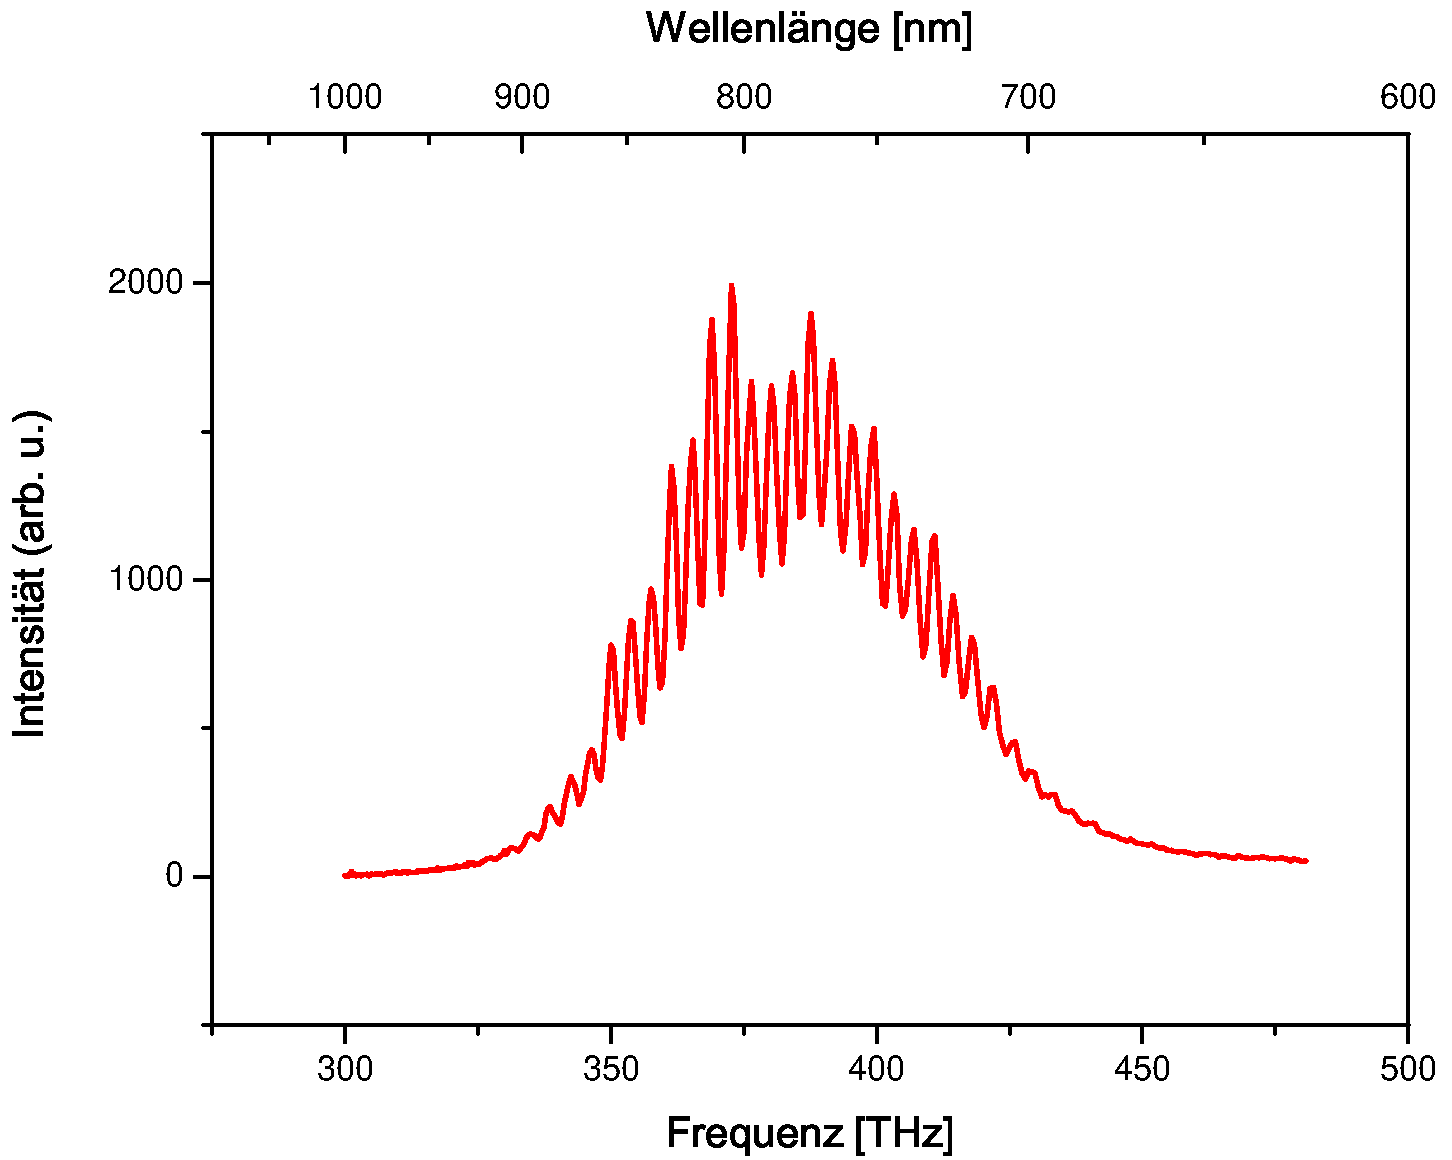
\includegraphics[width=0.49\textwidth]{figures/gratingEtalon}}
   \hfill
   \subfloat[Oszilloskop\label{fig:osziEtalon}]
   {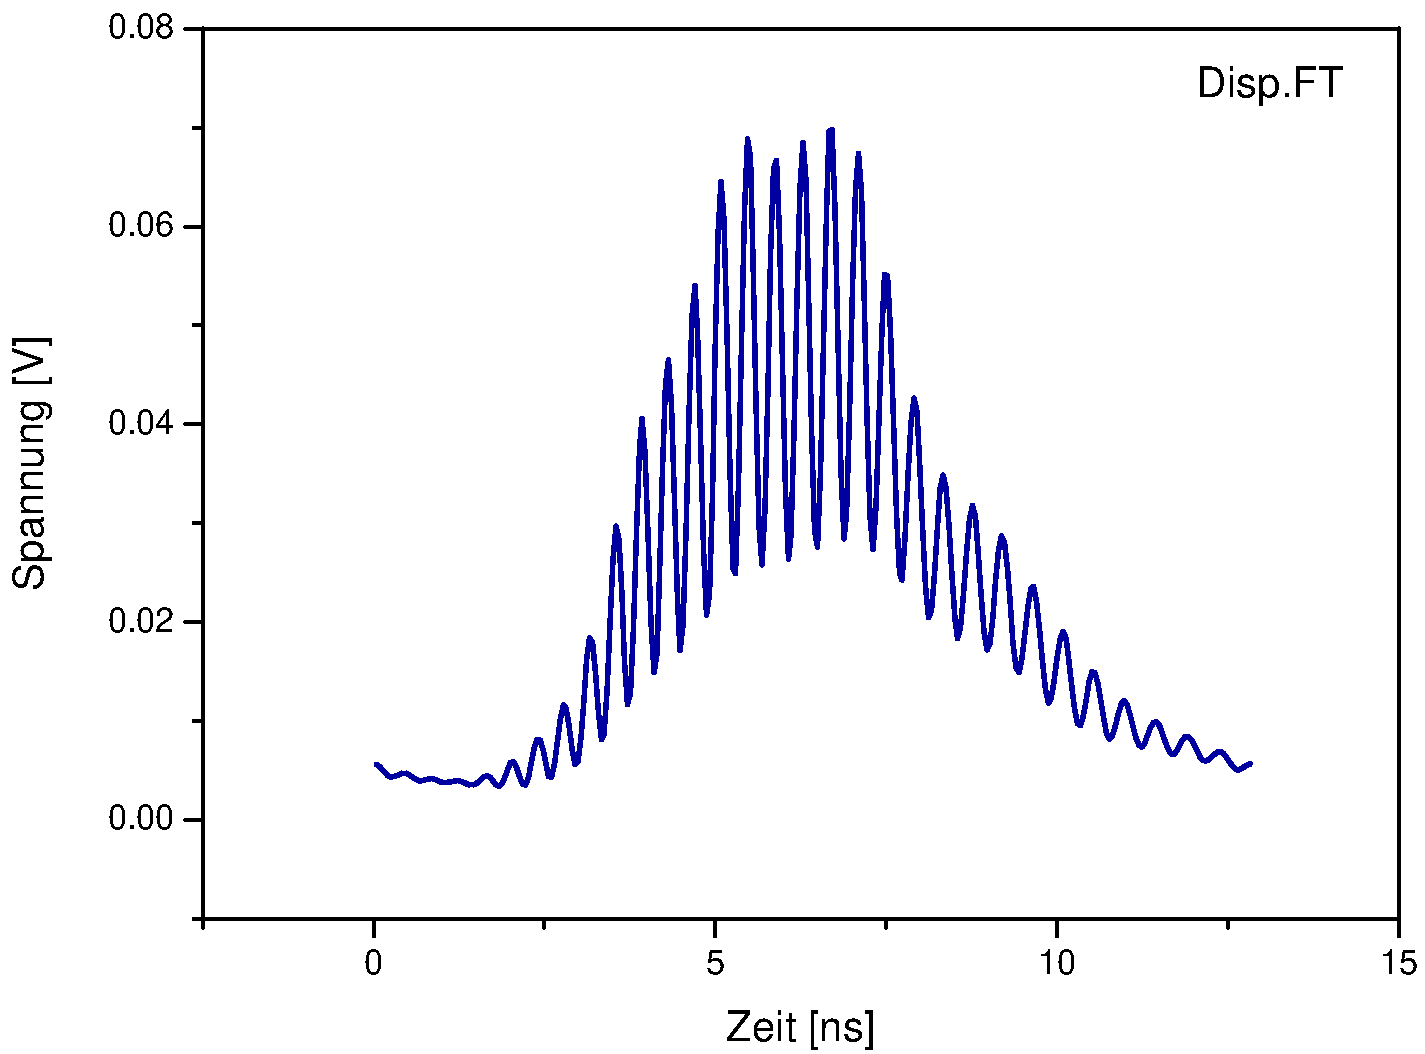
\includegraphics[width=0.49\textwidth]{figures/osziEtalon}}
   \hfill
   \subfloat[Kalibration\label{fig:calibration}]
   {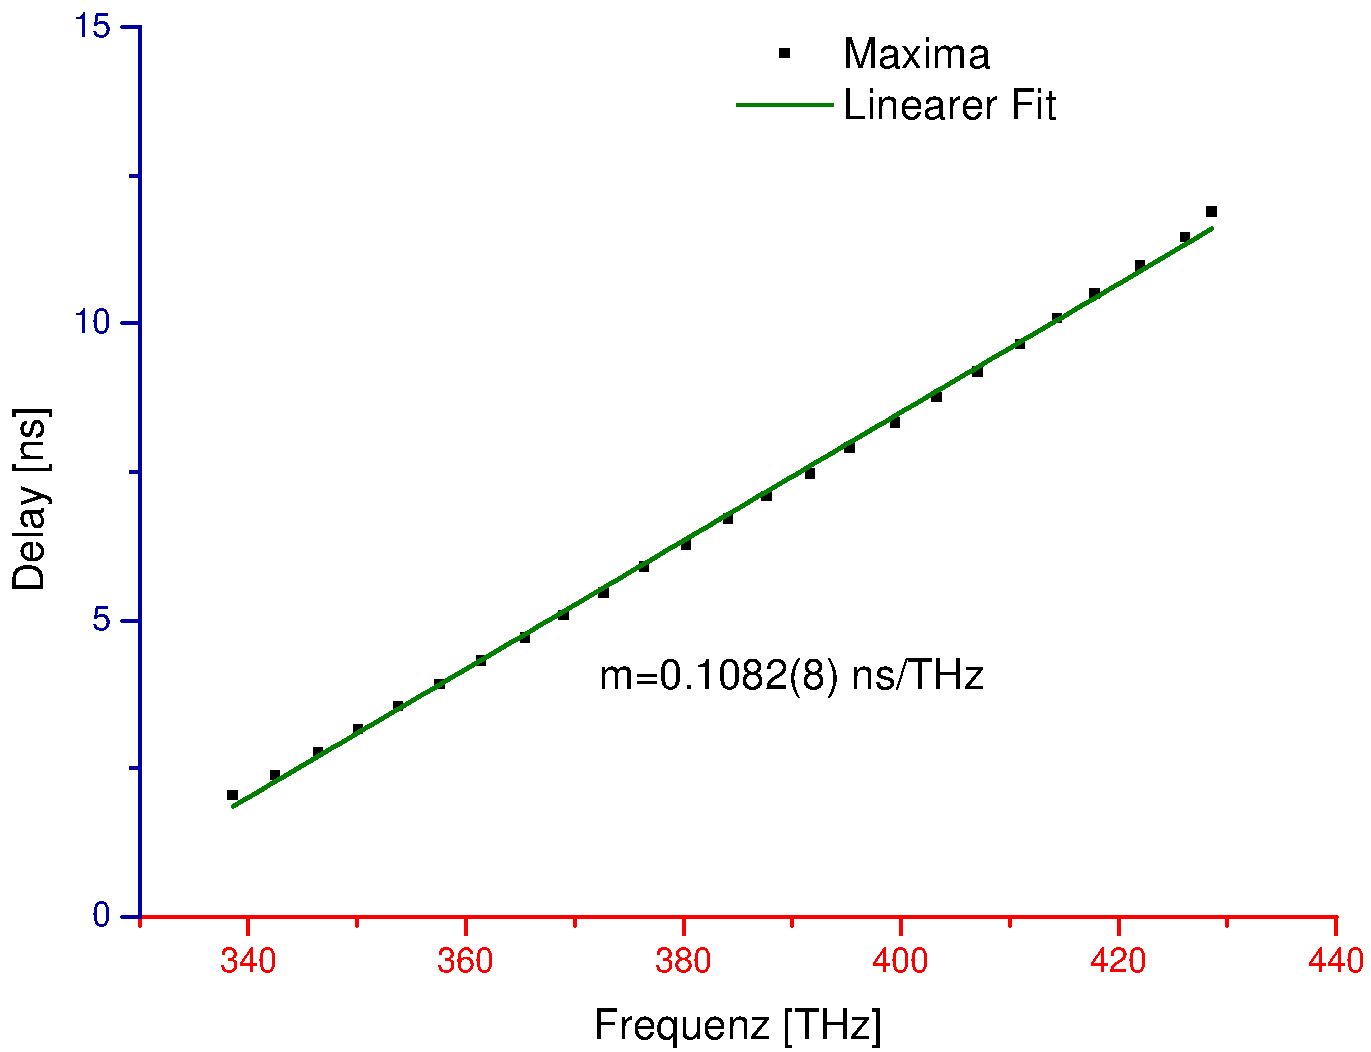
\includegraphics[width=0.6\textwidth]{figures/calibration}}
   \caption{Kalibration durch ein Etalon: Delay nach der Faser wird zu Frequenzen zugeordnet.}
   \label{fig:caliEtalon}
 \end{figure}

\section{Photodiode}
Als nächstes muss noch die Photodiode (Alphalas UPD-40-UVIR-P) charakterisiert werden.
\begin{table}[!htb]
	\centering
	\begin{tabular}{|c|c|}
		\hline
		Risetime & < 40\,ps \\
		Bandbreite & >8.5\,GHz \\
		Spektraler Bereich & 350-1700\,nm \\
		\hline	
	\end{tabular}
\end{table}
Zunächst wird getestet, in welchem Power-Bereich die Photodiode linear reagiert, damit man bei zukünftigen Messungen in diesem Bereich bleibt.
Dies muss für die beiden Modi undispergierter Puls sowie dispergiertes Signal geschehen.
Außerdem muss noch die Bandbreite der Photodiode abhängig von der eingestrahlten Leistung bestimmt werden, denn für die Beobachtung von relativ weit entfernten Pulsen (ca. 1\,ps) ist es wichtig, das die Photodiode schnell reagiert.
Diese Pulse sind zu nah, um sie im zeitlichen Signal getrennt zu sehen.
So kann man sie gerade noch als spektrale Interferenz wahrnehmen.
Das Spektrum sollte voll durchmoduliert sein, wenn beide Pulse gleich stark sind.
Die Photodiode wird jedoch ab einer bestimmten Modulationfrequenz, also einem bestimmten Abstand der Doppelpulse nicht so schnell reagieren können, dass das Signal komplett auf 0 heruntergeht.
Dadurch überschätzt man den Intensitätsunterschied der beiden Pulse.
\subsection{Undispergiert}
Man erkennt, dass die Peakamplitude bis ca. 2\,mW linear ansteigt.
Außerdem ist je nach Justage ein Ringing nach dem Puls zu beobachten.

\subsection{Dispergiert}
Bis ca. 10\,mW wächst das Signal linear.
Danach übersteuert man die Photodiode, sodass nicht genug Ladungsträger zwischen zwei Pulsen nachfließen können.

\subsection{Bandbreite}

\chapter{Ergebnisse}
Um durch eine langen Messung mit dem Oszilloskop die Entwicklung des Spektrums, etc. darstellen zu können, muss man erst die Pulswiederholrate bestimmen.
Dies geschieht über eine Fouriertransformation des ganzen Signals.
Die Frequenz des höchsten Peaks entspricht der Wiederholrate, das Inverse davon also dem Pulsabstand $t_\text{rep}$ bzw. der optischen Cavity-Länge des Lasers.
Da man diese zum Starten ändert, ist die bestimmte Wiederholrate nur für einen kurzen Ausschnitt der Messung korrekt.
Hat man also $t_\text{rep}$ bestimmt, legt man fest, in wie viele äquidistante Punkte man diese Zeit unterteilen möchte.
Dies sollte so gewählt sein, dass die Abstände in etwa zugehörigen Samplingrate entspricht.
Dann interpoliert man die Messdaten an den neuen Zeitpunkten und stellt die Daten anschließend als Matrix dar, trennt also jeden Roundtrip.
Die eine Achse entspricht den Roundtrips, die andere ist die Zeitachse pro Roundtrip.

Zuletzt muss man noch die Änderung der Repetitionsrate bzw. die Abweichung vom richtigen Wert korrigieren.
Dies kann auf zwei Arten geschehen:
Ist der Anteil an der Messung, bei der der Laser gemodelockt ist, groß, legt man ein Polynom durch die Peakpositionen des undispergierten, gemodelockten Signals, dehnt den Definitionsbereichs des Polynoms auf die gesamte Messung aus und verschiebt dann jeden Roundtrip so, dass diese Peakpositionen konstant sind.
Mit dem gleichen Polynom (nur mit einem anderen Offset) verschiebt man auch die dispergierte Messung.
Ist der Anteil an der Messung, bei der der Laser gemodelockt ist, jedoch kleiner, sodass man einen großen Fehler macht, wenn man das wie oben gefittete Polynom auch auf den nicht-gemodelockten Bereich ausdehnt, muss man sich einer anderen Methode bedienen, um die Änderung der Rep.rate zu korrigieren.
Dies basiert auf der Korrelation zwischen zwei Roundtrips, denn man davon ausgehen, dass sich zwischen zwei aufeinanderfolgenden Roundtrips kaum etwas ändert.
Man beginnt mit einem gemodelockten Spektrum und geht von diesem Spektrum zu früheren Roundtrips und bestimmt zu diesem die Korrelation.
Sollte der maximale Wert nicht bei der Verschiebung $\tau=0$ der beiden Signale zueinander sein, verschiebt man diesen Roundtrip um eben diesen Wert, sodass die Korrelation nun maximal bei $\tau=0$ ist.
Nun wird dieser Roundtrip (allerdings unverschoben) als neue Referenz genommen.
Das Spiel beginnt von vorne, es wird wieder die Korrelation zwischen diesem und vorigen Roundtrips gebildet, etc.
Allerdings wird die benötigte Verschiebung logischerweise aufsummiert.
Es hat sich als sinnvoll erwiesen, als Referenz nicht nur einen Roundtrip zu wählen, sondern die Mittlung über mehrere.
Das macht das Verfahren unsensibel gegenüber Rauschen in den Messdaten, die zu zu starken Verschiebungen führen.

Im folgenden soll zunächst die bei Variation der Pumpleistung untersucht werden.
Dies geschieht anhand zwei verschiedener Messreihen.
Danach folgen weitere Beobachtungen wie z.B. Tripletts.

\section{Doppelpulse Messreihe 1}
\subsection{Running ($P_\text{Pump}=4.39\dots4.47\,$W)}
In diesem Zustand ist die Pumpleistung so gering, dass zwar zwei Pulse durch den Laser laufen, diese aber einen großen Intensitätsunterschied haben, so dass sie unterschiedliche optische Weglängen haben und sich so auf einer Skala von 100\,ms gegeneinander verschieben.
In Abb. \ref{fig:rBF441} sieht man eine \textit{FastFrame}-Aufnahme dieses Betriebs.
Dabei wird auf den stärkeren Puls getriggert und im Gegensatz zu den anderen Aufnahmen ist dies keine kontinuierliche Messung, bei der man zu jedem Roundtrip Spektrum und zeitliches Signal aufnimmt.
Hier überspringt man sehr viele Pulse, damit man eine solch lange Zeit mit so einer gleich hohen Samplingrate aufnehmen kann.

Wenn man genau hinschaut erkennt man, dass die Relativgeschwindigkeit zwischen beiden Pulsen nur annähernd konstant ist.
Dies lässt sich auch in der Peak-Spannung des undispergierten Signals erkennen, welche proportional zur Pulsenergie ist.
So wird der schwache Puls die meiste Zeit schwächer während der starke stärker wird.
Dies führt zu einer Zunahme der Relativgeschwindigkeit.
Es gibt jedoch zwei Zeitpunkte zwischen zwei aufeinanderfolgenden Kollisionen,bei denen sich dieses Verhalten genau umgekehrt: Es findet ein Energietransfer vom stärkeren zum schwächeren Puls statt und die Relativgeschwindigkeit nimmt ab.
Dies lässt sich damit erklären, dass die beiden Pulse sich gerade dann im Laserkristall begegnen und so der schwächere Puls vom Kerr-Effekt durch den stärkeren profitiert.

\begin{figure}[!htb]
   \centering   
   \subfloat[\textit{FastFrame}-Aufnahme\label{fig:rBF441}]
   {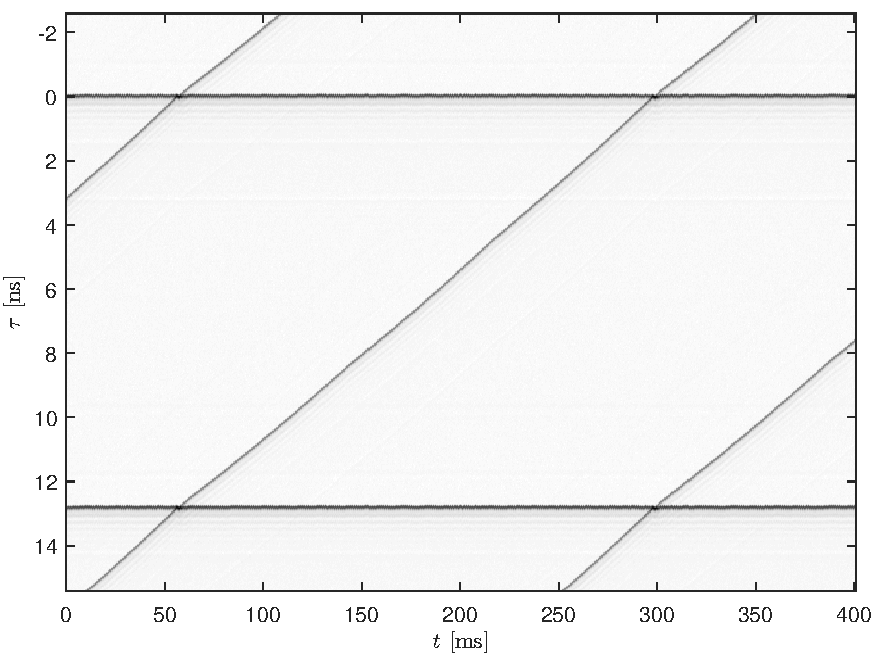
\includegraphics[width=0.49\textwidth]{figures/400ms_5musHold_25GSA_400m_MLrun_runBounceFix_4,41W_Ch2}}
   \hfill
   \subfloat[\label{fig:rBF441peakTau}]
   {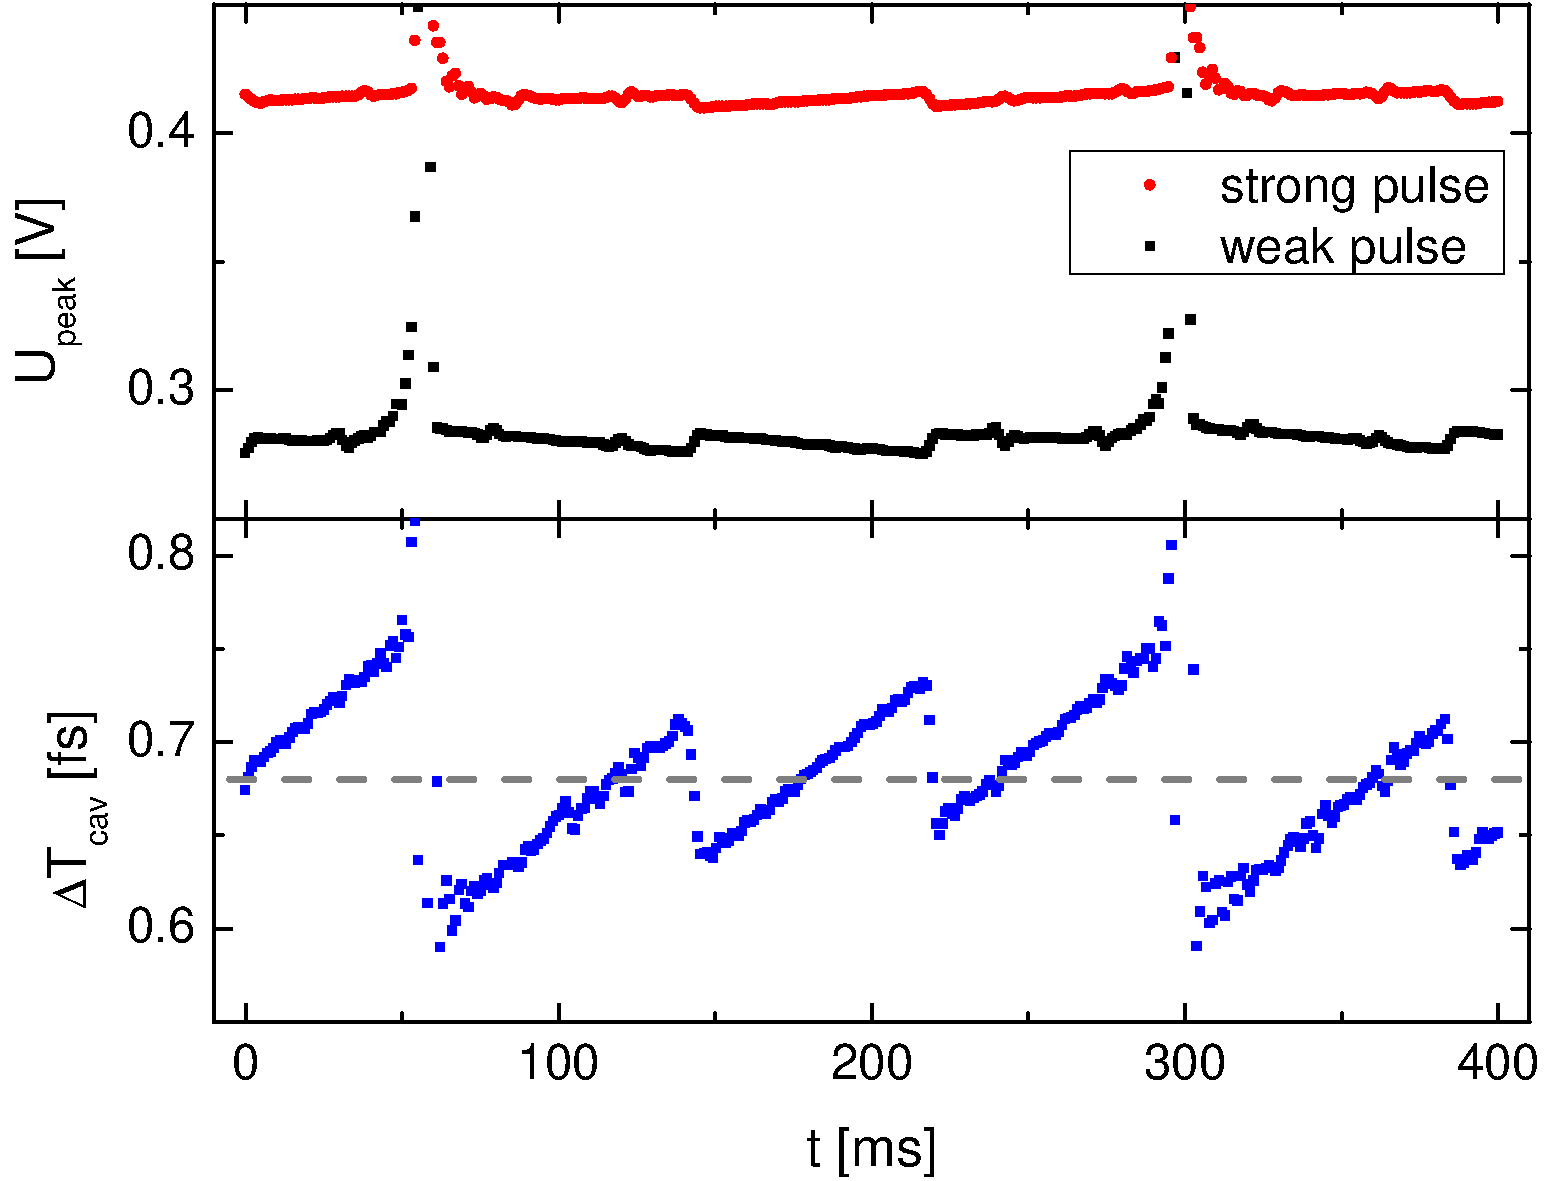
\includegraphics[width=0.49\textwidth]{figures/runningPeakTau}}
   \caption{Zwei unterschiedlich starke Pulse im Laser, die aufgrund des Kerr-Effekts verschiedene optische Weglängen sehen und sich so gegeneinander verschieben.}
   \label{fig:running441}
 \end{figure}

\subsection{Bouncing ($P_\text{Pump}=4.48\dots4.57\,$W)}
Dieser Zustand ist dadurch gekennzeichnet, dass es ständig zu Kollisionen zwischen den beiden Pulsen kommt, wie in Abbildung \ref{fig:rBF456} gut zu erkennen ist.
Diese entfernen sich danach schnell voneinander bevor der Abstand beider Pulse linear abnimmt und es schließlich zur erneuten Kollision kommt.
Erklären kann man dies damit, dass sich nach der Kollision ein schwacher Puls vor dem starken ausbildet, dieser aufgrund des Kerr-Effektes schneller durch die Cavity läuft und somit der Abstand beider größer wird.
Dann kommt es jedoch zu einem Erstarken des vorderen Pulses und zu einer Schwächung des hinteren, weil der hintere nur die schon vom vorderen reduzierte Besetzungsinversion sieht und so weniger Verstärkung bekommt.
Es stellt sich ein fixes Intensitätsverhältnis und somit auch eine konstante Relativgeschwindigkeit ein, sodass sich beide mit dieser annähern bis es zur nächsten Kollision kommt.
Somit lässt sich auch erklären, warum die Kollisionszeit $T_\text{interColl.}$, also die Zeit zwischen zwei Kollisionen linear mit der maximalen Entfernung $\tau_\text{max}$ zusammenhängt (Abb. \ref{fig:bounceDistTime}).

\begin{figure}[!htb]
   \centering   
   \subfloat[Ausschnitt der Autokorrelation\label{fig:rBF456}]
   {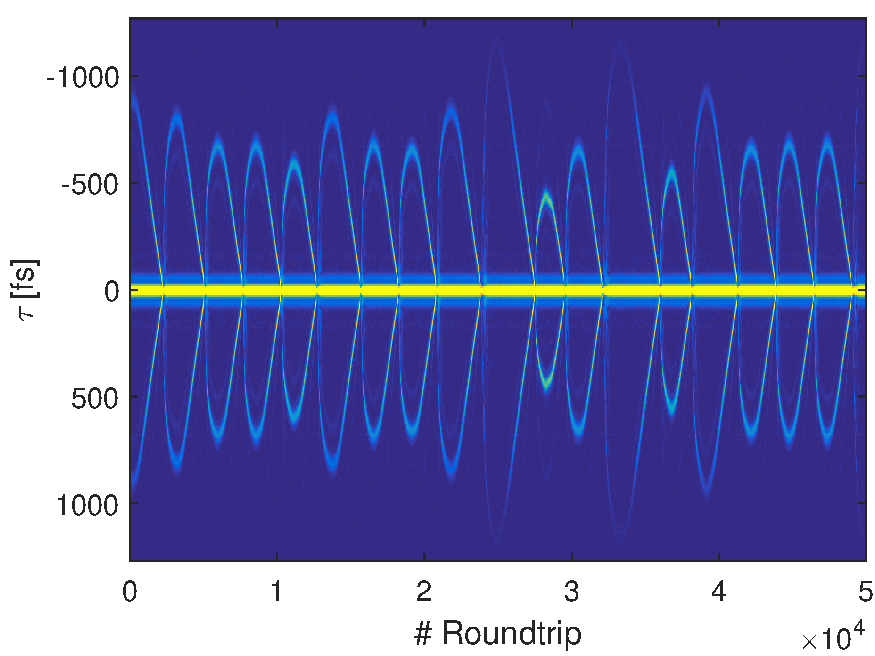
\includegraphics[width=0.49\textwidth]{figures/4ms_25GSA_400m_MLrun_runBounceFix_4,56W_Ch1_100000_150000_autocorr}}
   \hfill
   \subfloat[Histogramm des maximalen Abstandes $\tau_\text{max}$ der beiden Pulse pro Bounce\label{fig:rBF456histo}]
   {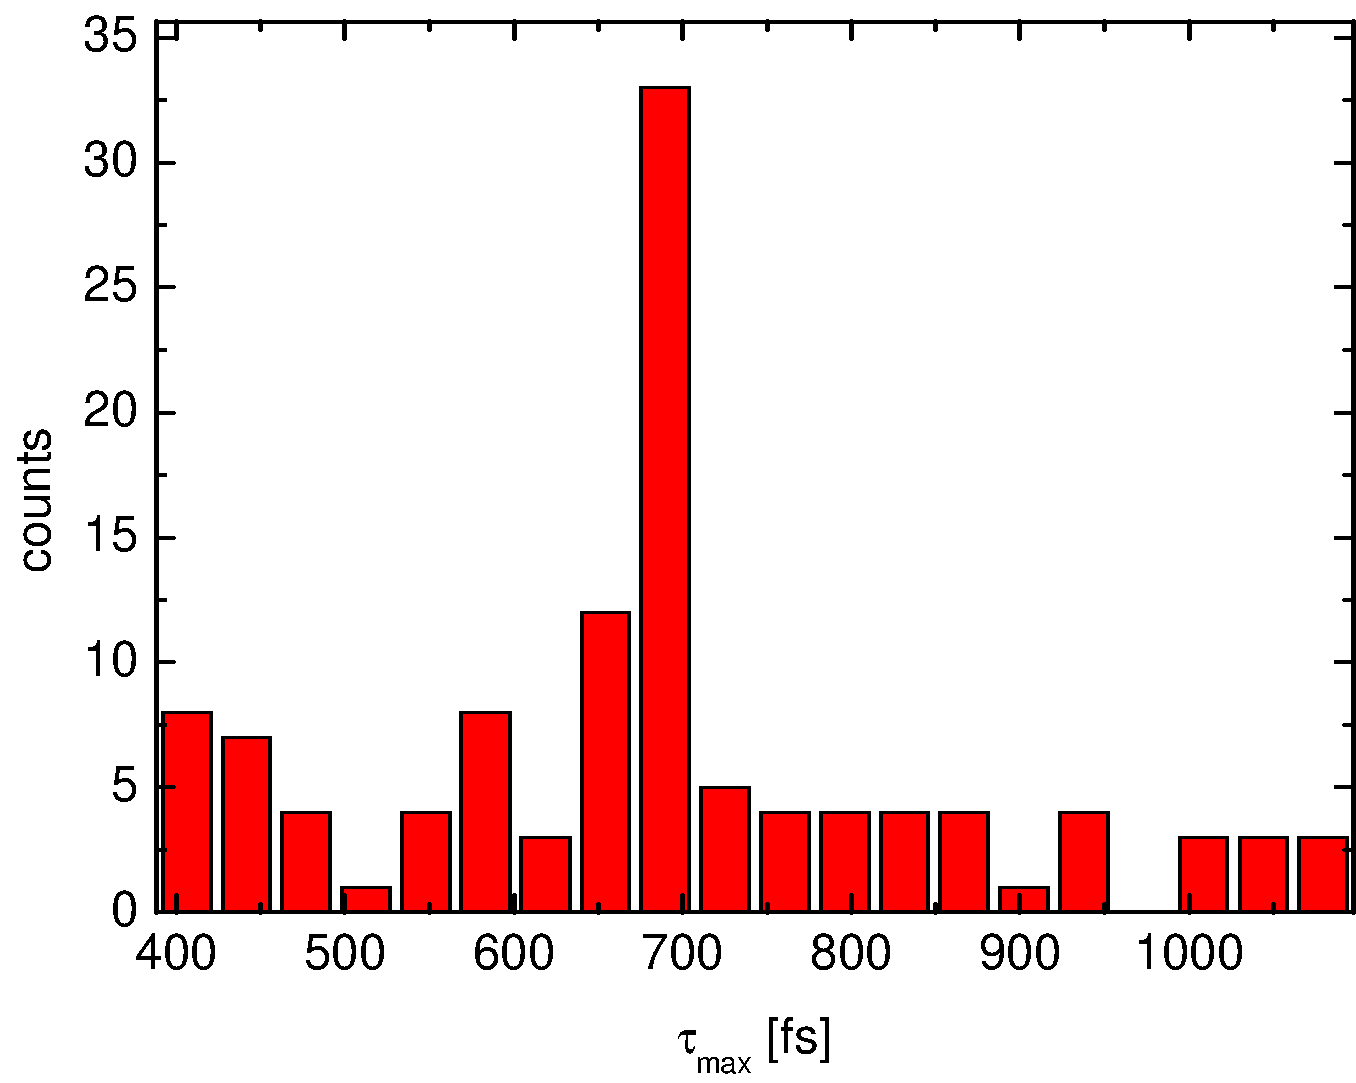
\includegraphics[width=0.49\textwidth]{figures/bounce456histo}}
   \caption{Bouncing-Mode bei einer Pumpleistung von $4.56\,$W.}
   \label{fig:bouncing456}
 \end{figure}

Wenn man die Pumpleistung auf 4.57\,W erhöht, sieht man noch einen weiteren Interaktionsmechanismus: Die beiden Pulse stoßen sich voneinander ab, bevor sie überhaupt kollidieren.

\begin{figure}[!htb]
   \centering
   \subfloat[Überblick.\label{fig:rBF457_autocorr}]
   {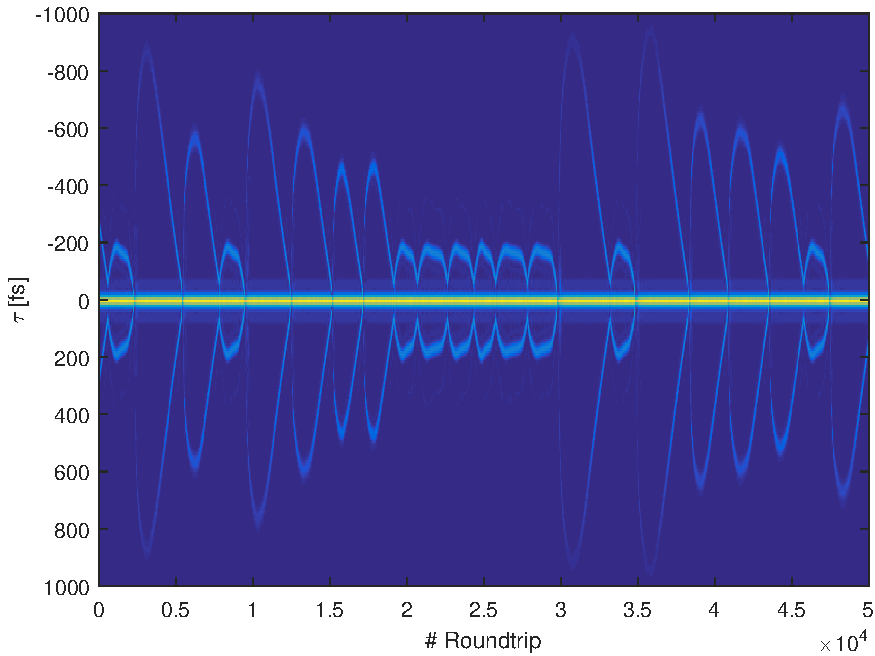
\includegraphics[width=0.49\textwidth]{figures/4ms_25GSA_400m_MLrun_runBounceFix_4,57W_Ch1_120000_170000_autocorr}}
   \hfill
   \subfloat[Zoom.\label{fig:rBF457_autocorr_zoom}]
   {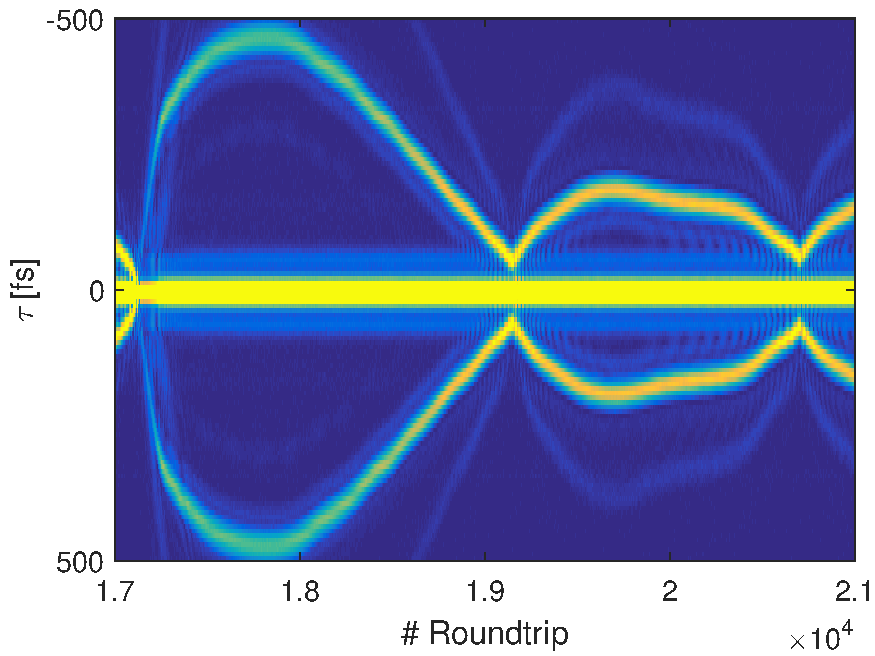
\includegraphics[width=0.49\textwidth]{figures/4ms_25GSA_400m_MLrun_runBounceFix_4,57W_Ch1_137000_141000_autocorr}}
   
   \subfloat[Abstoßung, spektrale Ansicht.\label{fig:rBF457_repel_spec}]
   {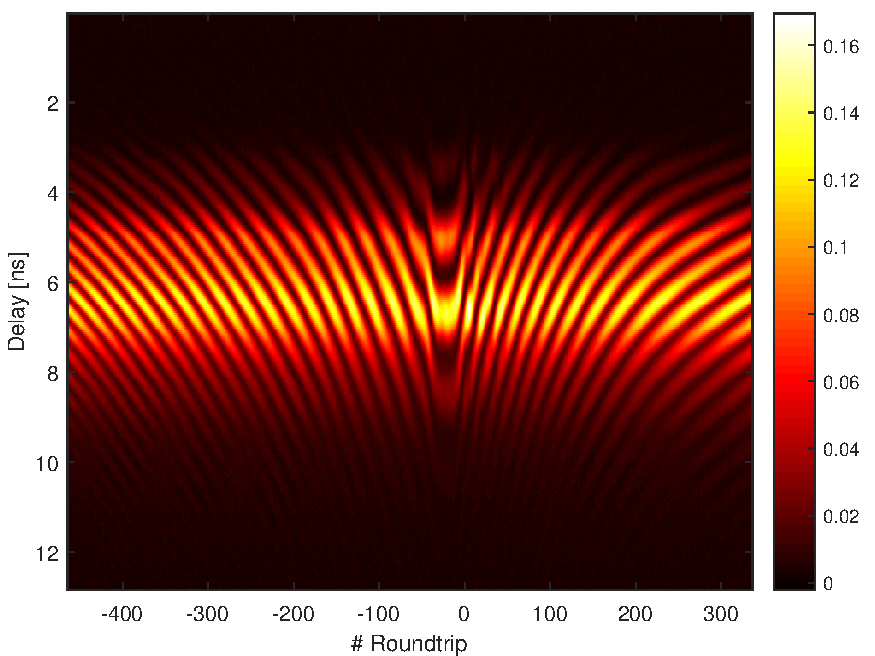
\includegraphics[width=0.49\textwidth]{figures/4ms_25GSA_400m_MLrun_runBounceFix_4,57W_Ch1_138700_139500_spectrum}}
   \hfill
   \subfloat[Abstoßung, Autokorrelation.\label{fig:rBF457_repel_autocorr}]
   {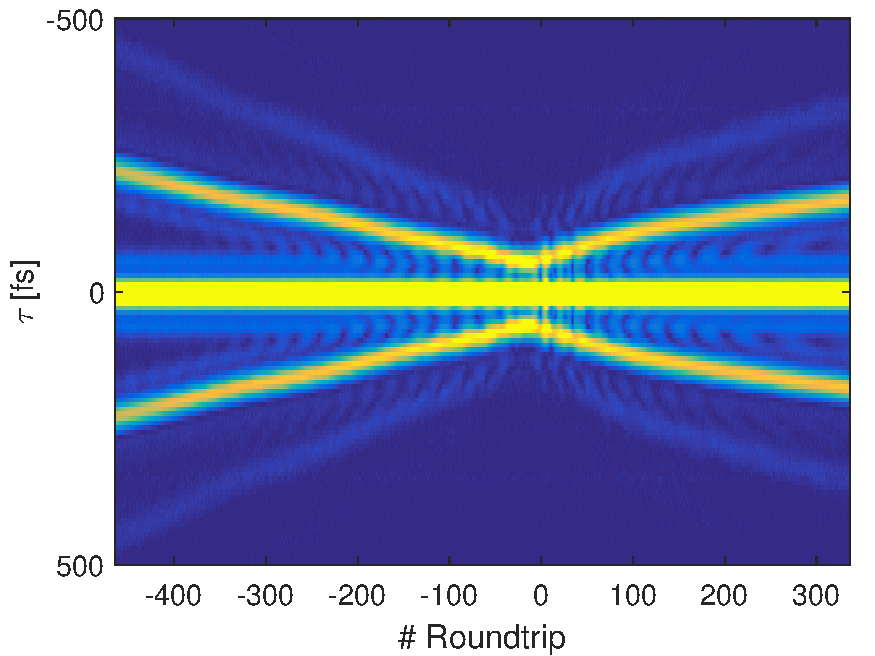
\includegraphics[width=0.49\textwidth]{figures/4ms_25GSA_400m_MLrun_runBounceFix_4,57W_Ch1_138700_139500_autocorr}}
   
   \subfloat[Kollision, spektrale Ansicht.\label{fig:rBF457_coll_spec}]
   {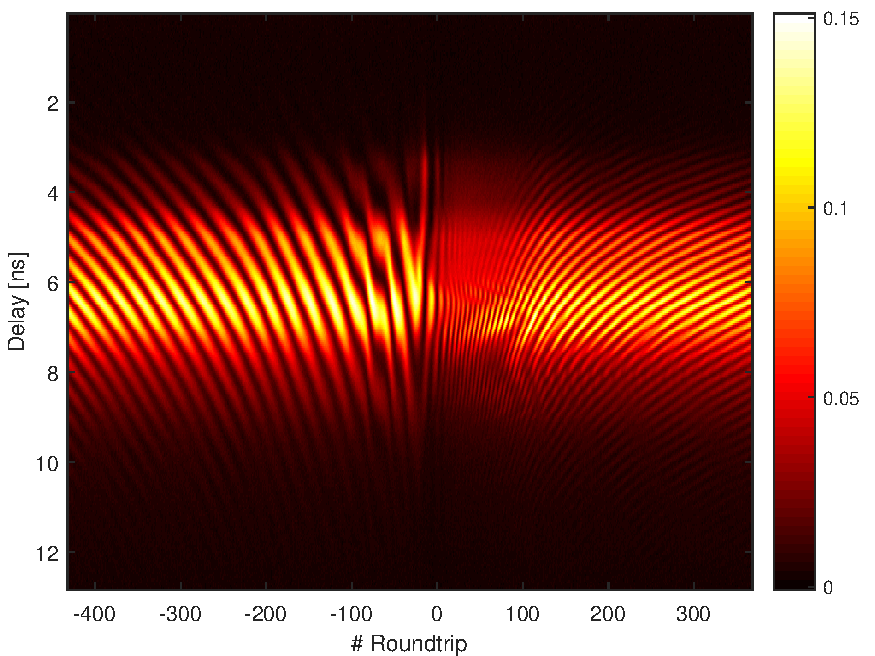
\includegraphics[width=0.49\textwidth]{figures/4ms_25GSA_400m_MLrun_runBounceFix_4,57W_Ch1_136700_137500_spectrum}}
   \hfill
   \subfloat[Kollision, Autokorellation.\label{fig:rBF457_coll_autocorr}]
   {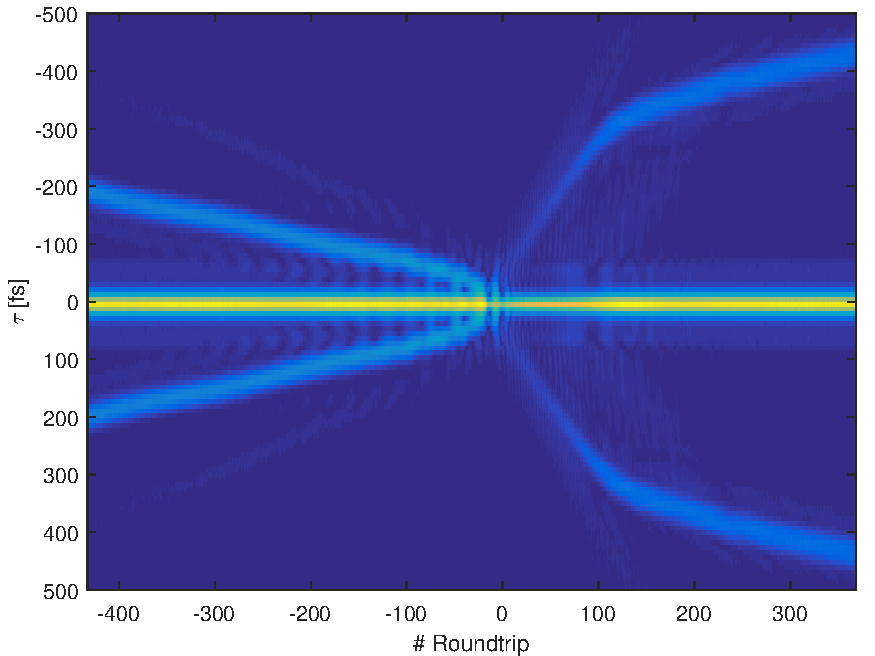
\includegraphics[width=0.49\textwidth]{figures/4ms_25GSA_400m_MLrun_runBounceFix_4,57W_Ch1_136700_137500_autocorr}}
   \caption{$P_\text{Pump}=4.57\,$W: Unterschied zwischen Kollision und Abstoßung der beiden Pulse.}
   \label{fig:rbf457}
 \end{figure}

\begin{figure}[!htb]
	\centering
	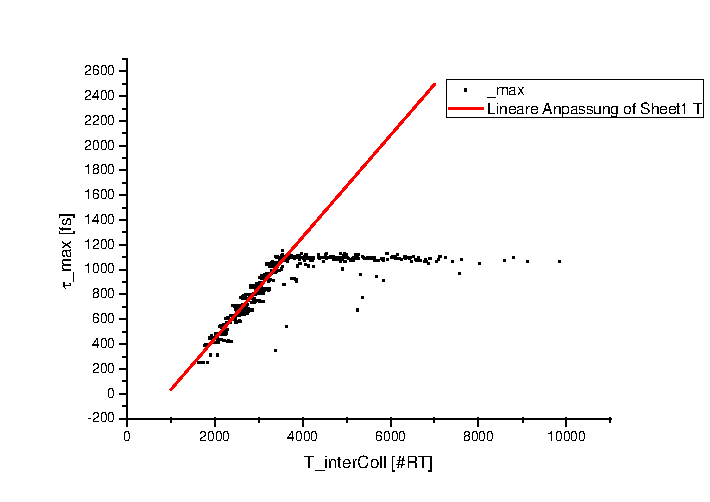
\includegraphics[width=0.8\textwidth]{figures/bounceDistTime}
	\caption{Maximaler Pulsabstand $\tau_\text{max}$ versus Zeit zwischen zwischen zwei Kollisionen $T_\text{interColl.}$. Das bestimmte $\tau_\text{max}$ ist begrenzt durch die maximale Modulationsfrequenz des Spektrums.}
	\label{fig:bounceDistTime}
\end{figure}

\subsection{Bound Solitons ($P_\text{Pump}=4.57\dots4.81\,$W)}
In diesem Zustand ändert sich der Abstand der Pulse nicht gravierend.
Es gibt jedoch ein oszillatorisches Verhalten der Phase und des Abstandes.
Für drei der in Abbildung \ref{fig:boundSpectro} gezeigten Messreihen ist dieses Verhalten in die \textit{Interaction Plane} eingezeichnet, also ein polarer Plot mit dem Abstand als Radius und der Phase als Winkel.
In Abbildung \ref{fig:interactionPlane} ist jedoch der Radius der um 80\,fs verringerte Abstand, damit man Abstandsänderungen gut erkennen kann.
Zusätzlich sind Pfeile eingezeichnet, die anzeigen in welche Richtung die Orbits durchlaufen werden.
\begin{figure}[!htb]
   \centering
   \subfloat[\label{fig:rBF458}]
   {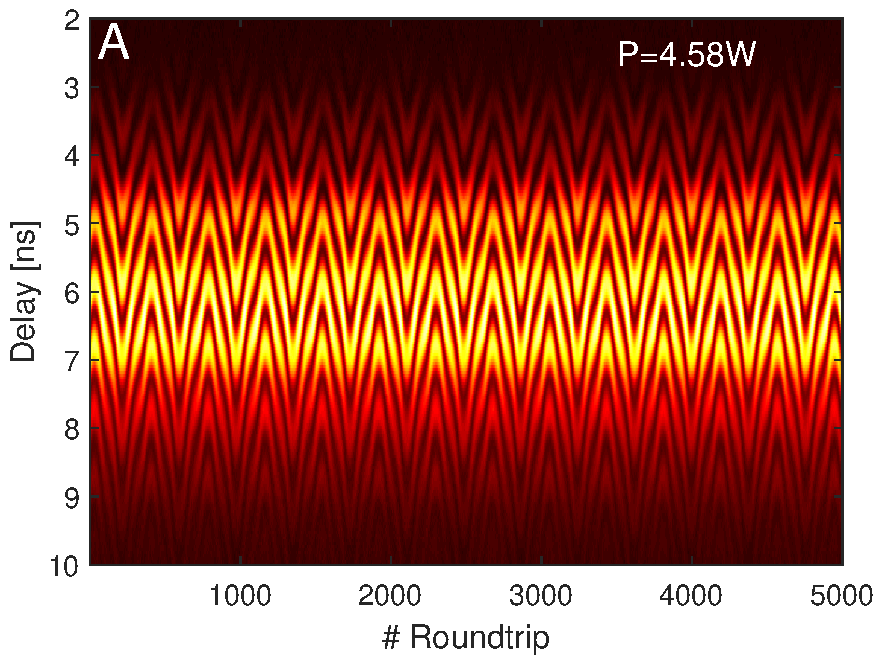
\includegraphics[width=0.49\textwidth]{figures/4ms_25GSA_400m_MLrun_runBounceFix_4,58W_Ch_PWnoCB}}
   \hfill
   \subfloat[\label{fig:rBF463}]
   {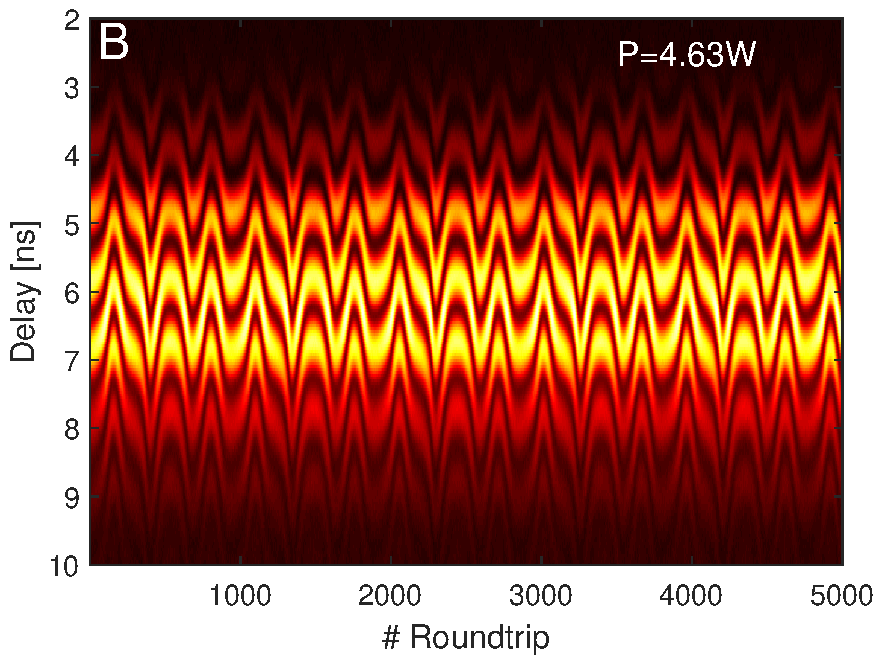
\includegraphics[width=0.49\textwidth]{figures/4ms_25GSA_400m_MLrun_runBounceFix_4,63W_Ch_PWnoCB}}
   
   \subfloat[\label{fig:rBF464}]
   {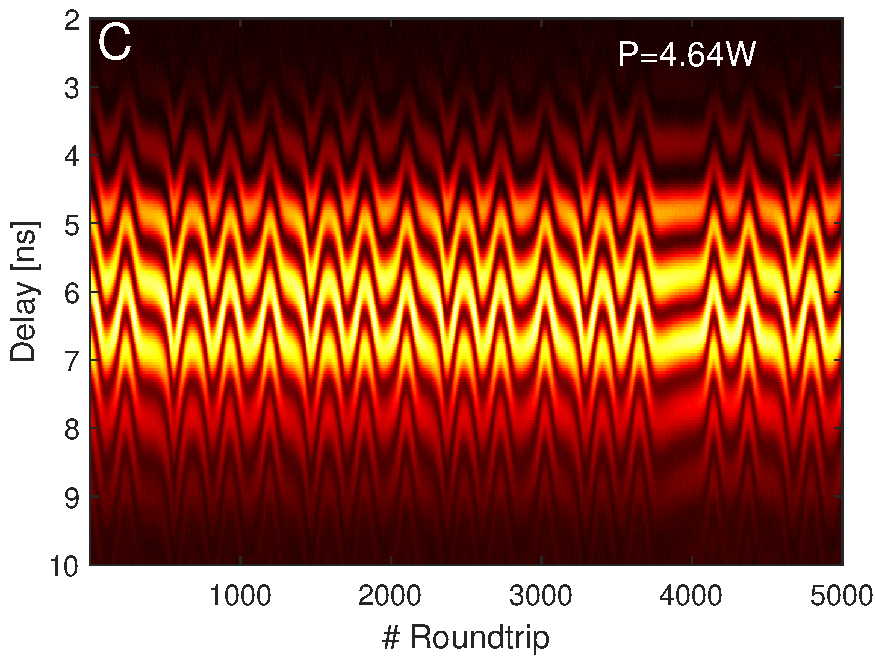
\includegraphics[width=0.49\textwidth]{figures/4ms_25GSA_400m_MLrun_runBounceFix_4,64W_Ch_PWnoCB}}
   \hfill
   \subfloat[\label{fig:rBF468}]
   {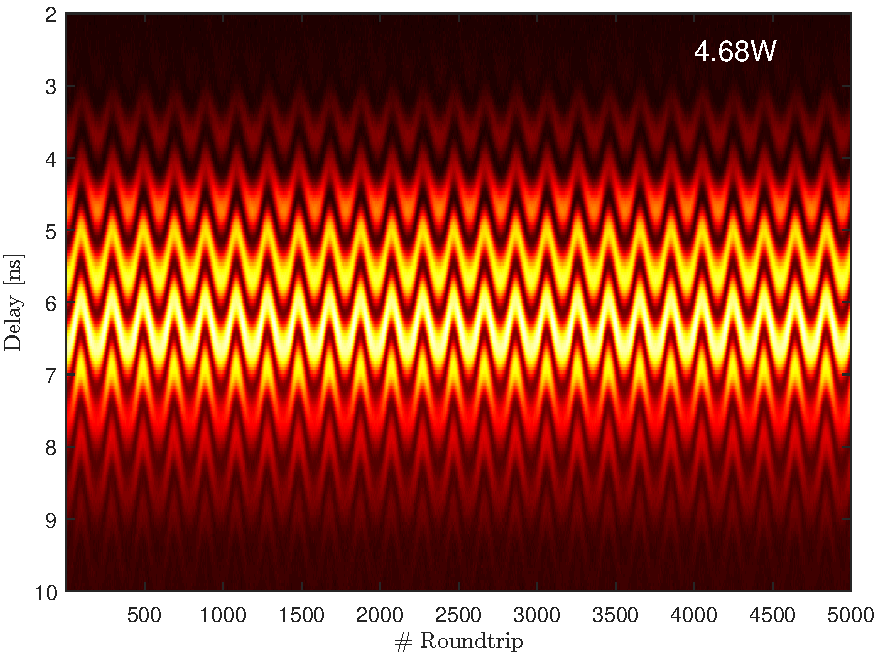
\includegraphics[width=0.49\textwidth]{figures/4ms_25GSA_400m_MLrun_runBounceFix_4,68W_Ch_PWnoCB}}
   \caption{Bound Solitons: Spektren bei Änderung der Pumpleistung.}
   \label{fig:boundSpectro}
 \end{figure}
 
 \begin{figure}[!htb]
	\centering
	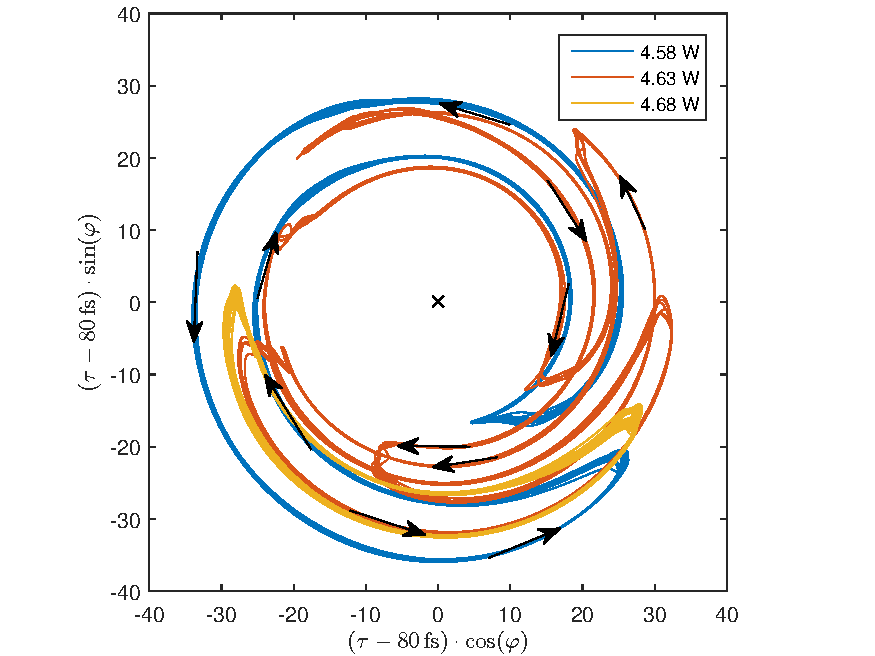
\includegraphics[width=0.8\textwidth]{figures/4ms_25GSA_400m_MLrun_runBounceFix_InteractionPlaneArrows2.pdf}
	\caption{Phasendynamik in der Interaction Plane.}
	\label{fig:interactionPlane}
\end{figure}

\section{Doppelpulse Messreihe 2}
Hier beginnt man mit Doppelpulsen, deren Phase und relativer Abstand fix sind.
Der Abstand liegt etwa bei 170 \,fs.
Dann dreht man die Pumpleistung herunter.
Dabei beobachtet man, dass der Abstand der beiden Pulse immer noch sehr konstant ist, während die Phase jedoch beginnt, durchzulaufen.
Dies deutet auf einen Intensitätsunterschied zwischen beiden Pulsen hin.
Die Phase läuft jedoch nicht linear durch, sondern bildet Stufen.
Nach XXX ist die Phase bei $\varphi=\pm\pi/2$ gelockt.
Vermutlich kann in der Umgebung von diesem Wert die fehlende Energie noch durch Senkung beider Pulsamplituden aufgefangen werden, was zu einer annähernd konstanten Phase führt, wohingegen diese ab einer bestimmten Abweichung von $\pi/2$ sich in sehr kurzer Zeit um fast $2\pi$ ändert.
Dies könnte bedeuten, dass dann der vordere sehr schnell stärker und der hintere schwächer wird, bis die Phase erneut etwas kleiner als $\pi/2$ ist und beide Pulse ihre Amplituden angleichen.
Verringert man die Pumpleistung weiter, geschieht dieser Prozess schneller, bis die Phase annähernd linear durchläuft.
\begin{figure}[!htb]
   \centering
   \captionsetup[subfigure]{labelformat=empty}
   \captionsetup[subfloat]{farskip=-10pt,captionskip=0pt}
   \subfloat[]{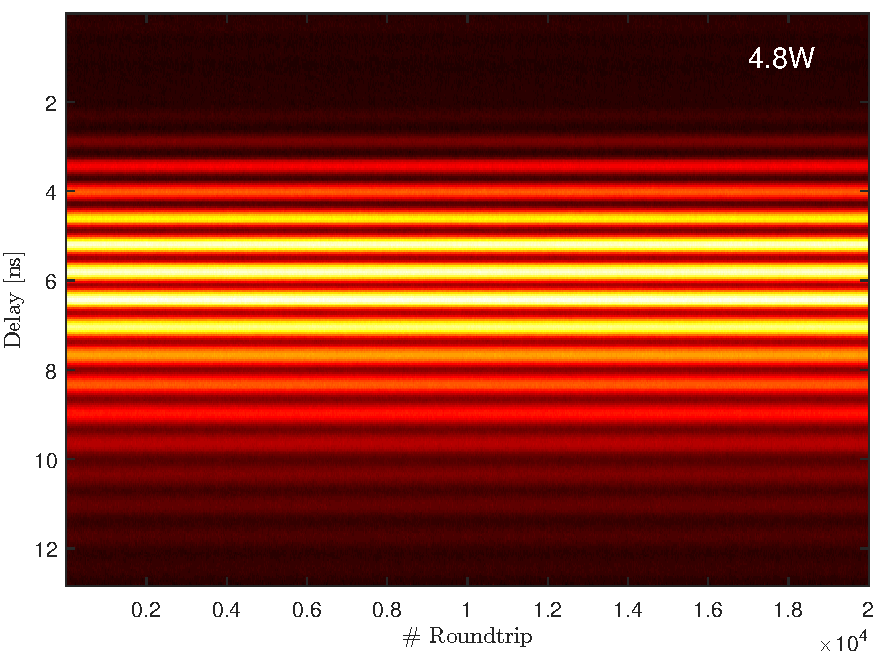
\includegraphics[width=0.49\textwidth]{figures/4ms_25GSA_400m_MLrun_Doppel4,8W_2_Ch_PWnoCB}}
   \hfill
   \subfloat[]
   {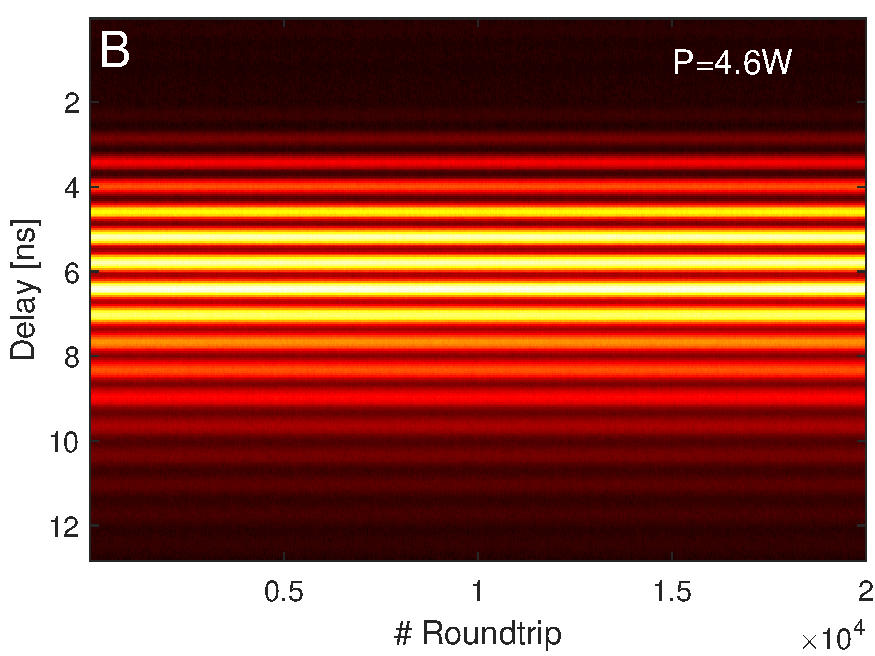
\includegraphics[width=0.49\textwidth]{figures/4ms_25GSA_400m_MLrun_Doppel4,6W_Ch_PWnoCB}}
   %\hfill
   
   \subfloat[]
   {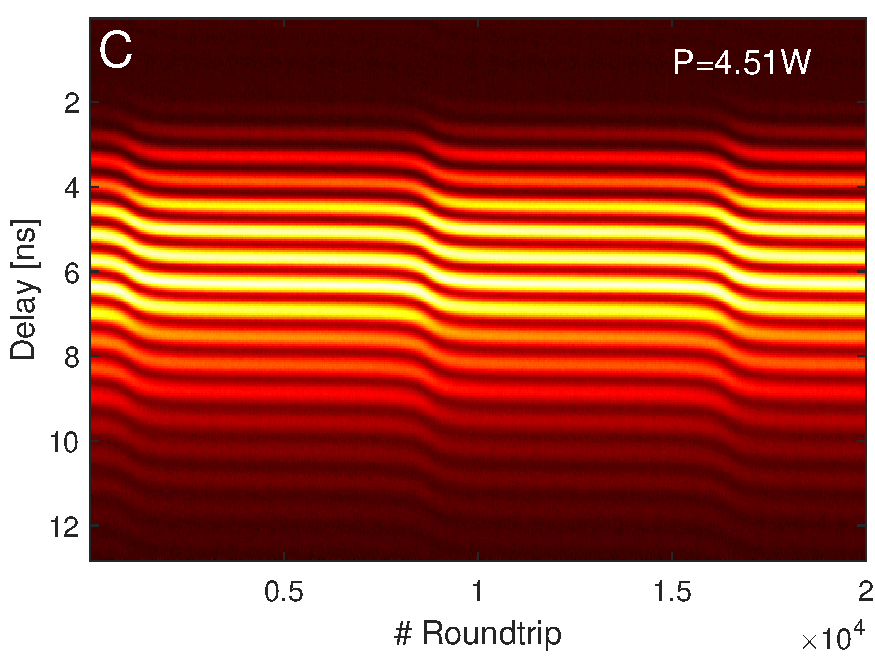
\includegraphics[width=0.49\textwidth]{figures/4ms_25GSA_400m_MLrun_Doppel4,51W_Ch_PWnoCB}}
   \hfill
   \subfloat[]
   {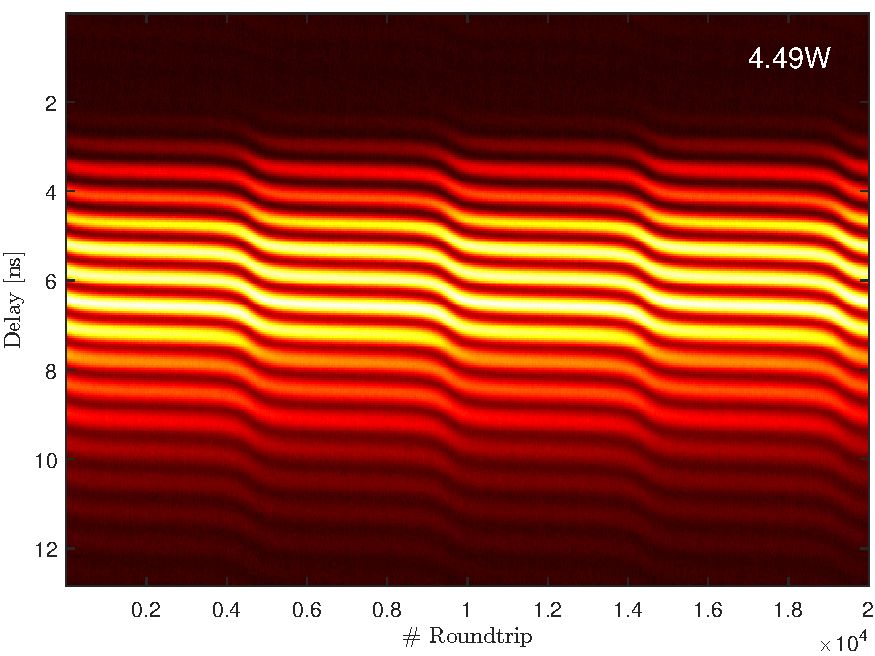
\includegraphics[width=0.49\textwidth]{figures/4ms_25GSA_400m_MLrun_Doppel4,49W_Ch_PWnoCB}}
   %\hfill
   
   \subfloat[]
   {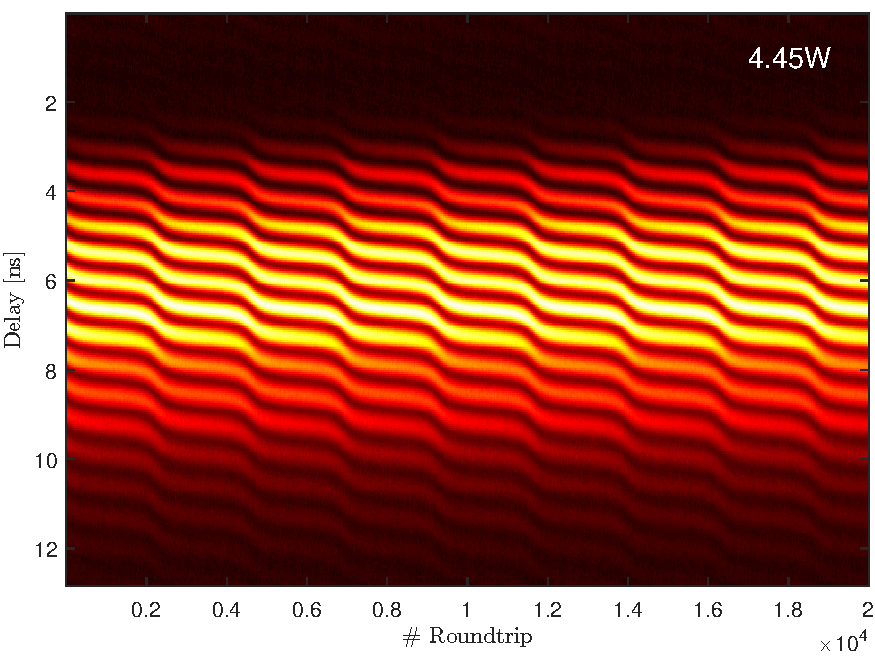
\includegraphics[width=0.49\textwidth]{figures/4ms_25GSA_400m_MLrun_Doppel4,45W_2_Ch_PWnoCB}}
   \hfill
   \subfloat[]
   {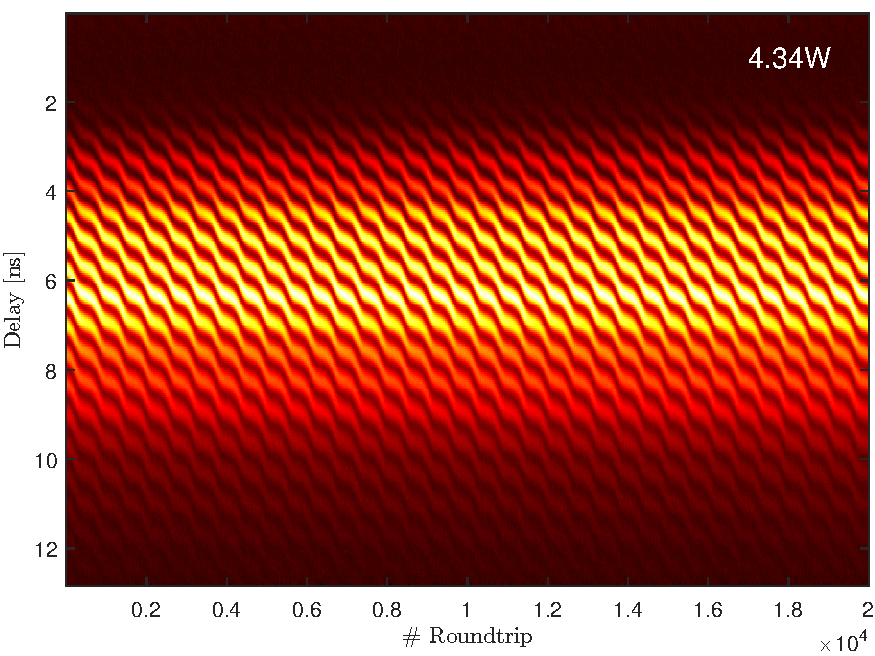
\includegraphics[width=0.49\textwidth]{figures/4ms_25GSA_400m_MLrun_Doppel4,34W_Ch_PWnoCB}}
   %\hfill
   
   \subfloat[]
   {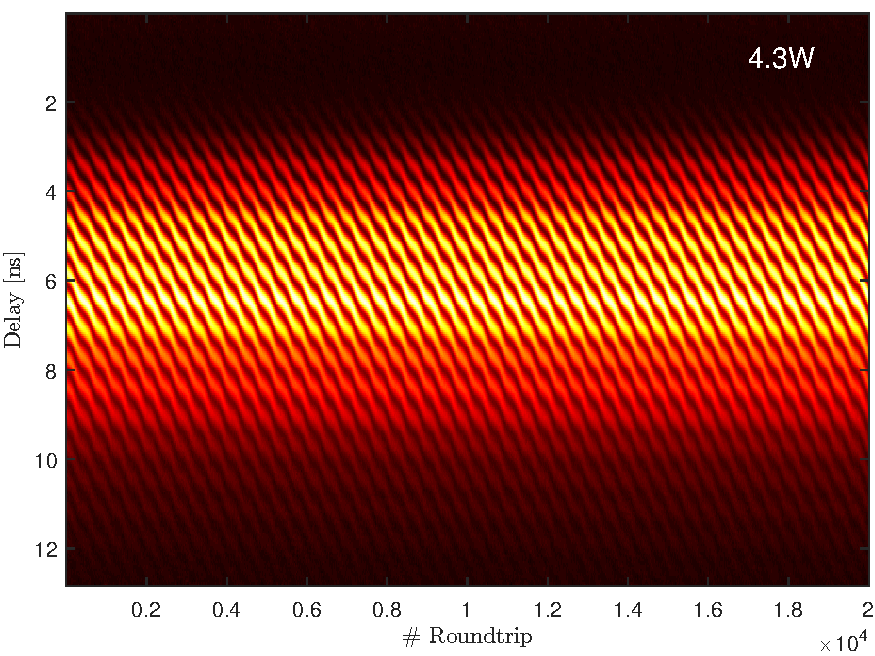
\includegraphics[width=0.49\textwidth]{figures/4ms_25GSA_400m_MLrun_Doppel4,3W_Ch_PWnoCB}}
   \hfill
   \subfloat[]
   {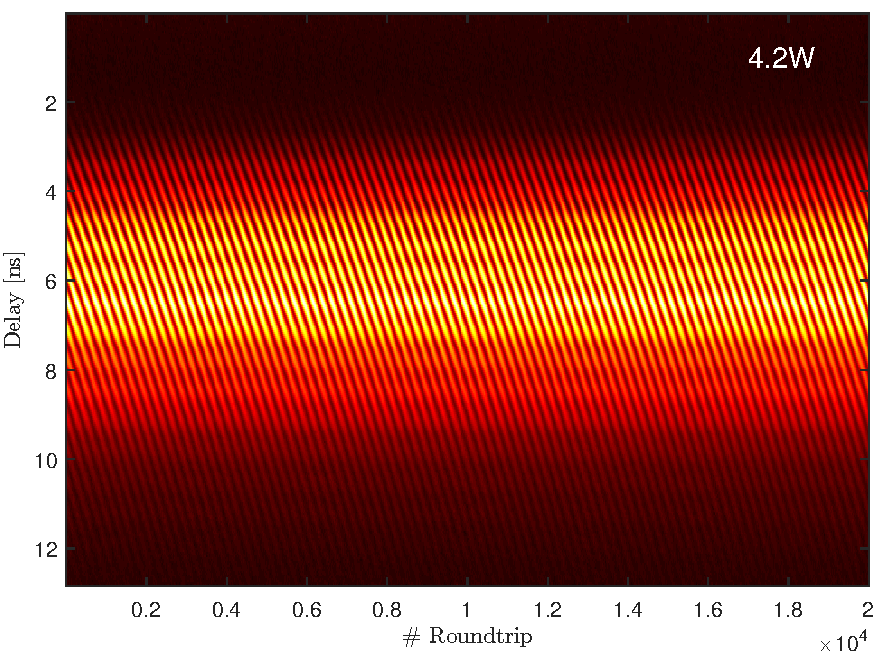
\includegraphics[width=0.49\textwidth]{figures/4ms_25GSA_400m_MLrun_Doppel4,2W_Ch_PWnoCB}}
   \caption{Verringerung der Pumpleistung: Von einer festen Phase über Stufen zu einer annähernd linear durchlaufenden Phase.}
   \label{fig:165014steps}
 \end{figure}
 
% \begin{figure}[!htb]
%   \centering
%   \captionsetup[subfigure]{labelformat=empty}
%   \captionsetup[subfloat]{farskip=-10pt,captionskip=0pt}
%   \subfloat[]
%   {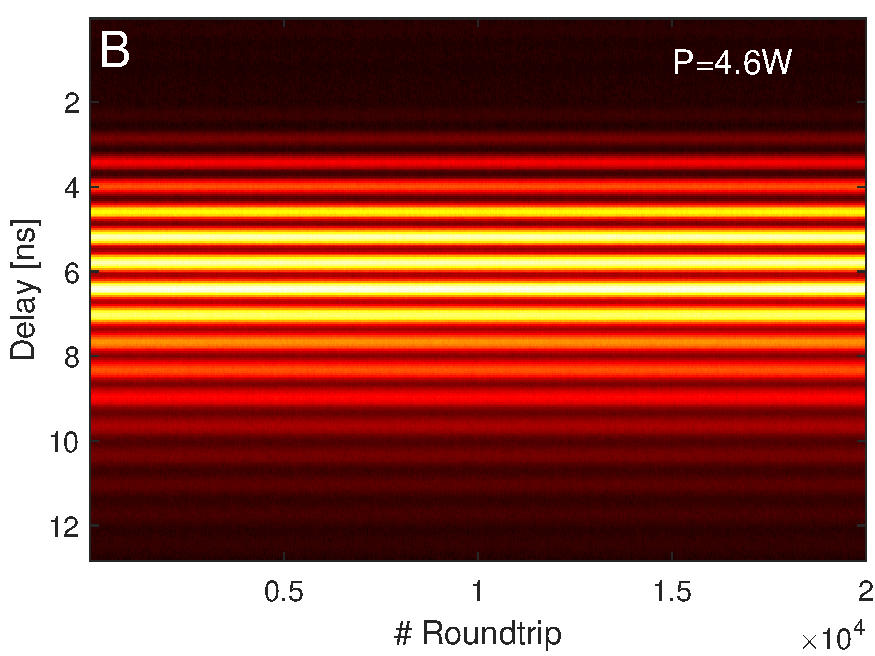
\includegraphics[width=0.49\textwidth]{figures/4ms_25GSA_400m_MLrun_Doppel4,6W_Ch_PWnoCB}}
%   \hfill
%   \subfloat[]
%   {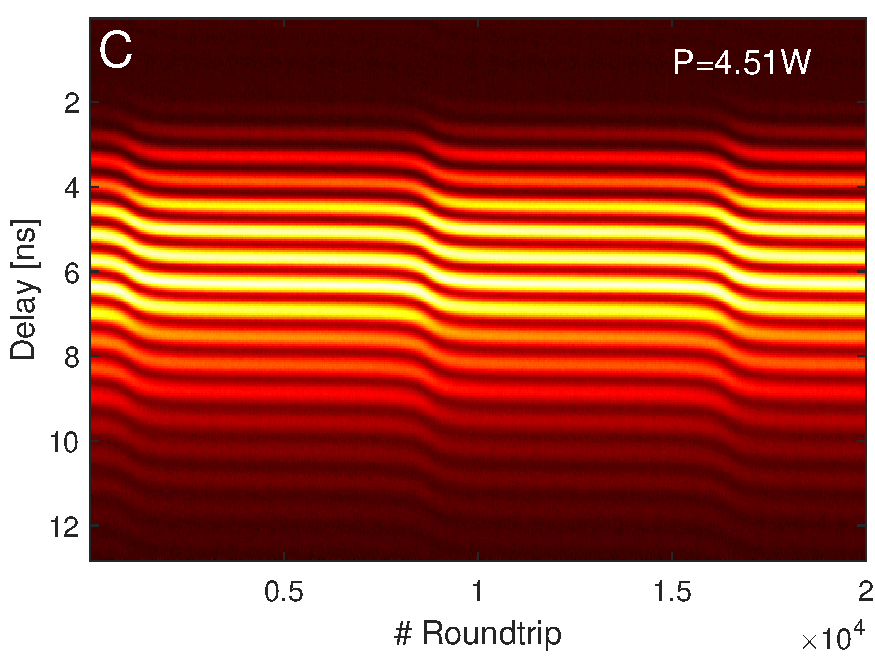
\includegraphics[width=0.49\textwidth]{figures/4ms_25GSA_400m_MLrun_Doppel4,51W_Ch_PWnoCB}}
%   
%   \subfloat[]
%   {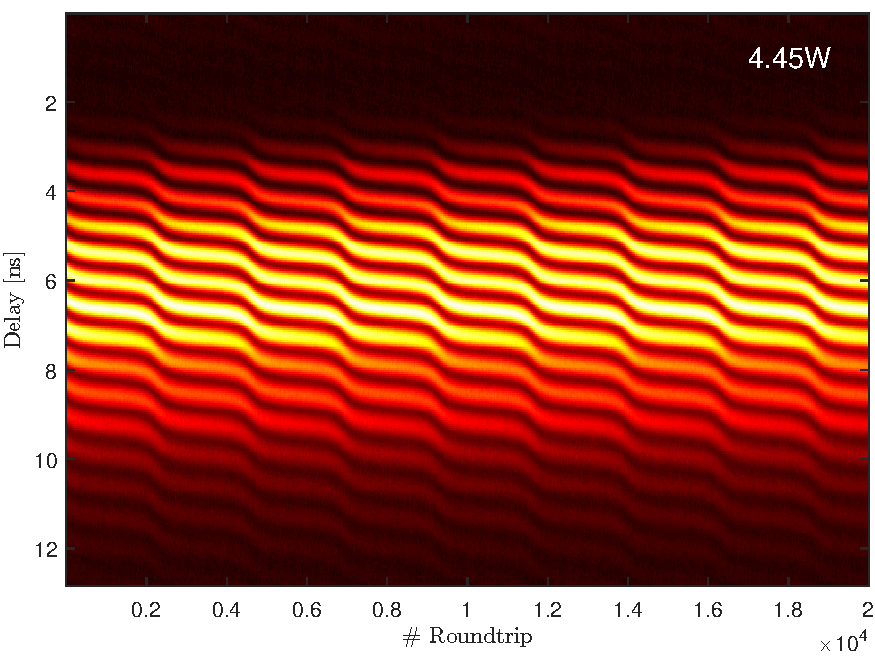
\includegraphics[width=0.49\textwidth]{figures/4ms_25GSA_400m_MLrun_Doppel4,45W_2_Ch_PWnoCB}}
%   \hfill
%   \subfloat[]
%   {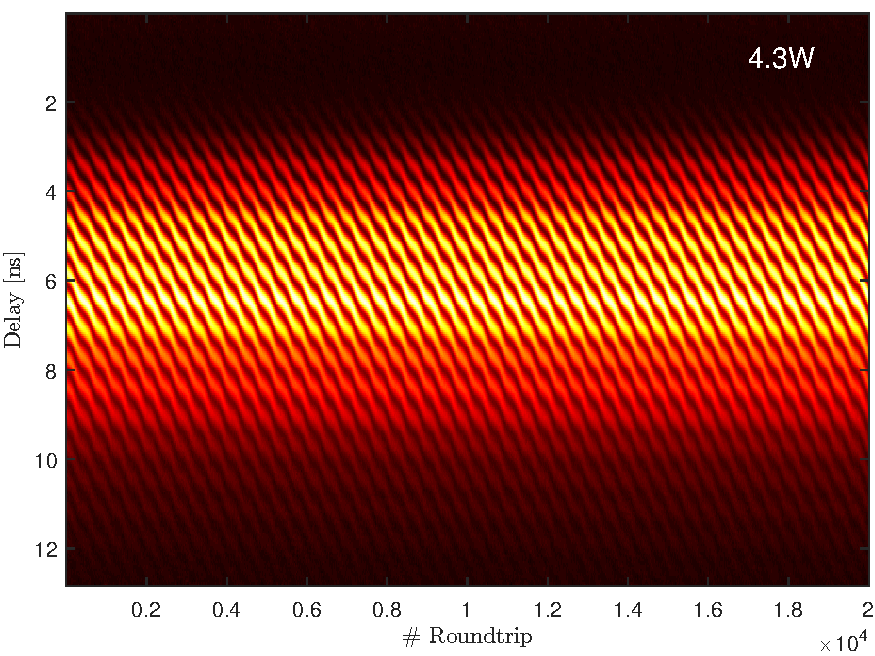
\includegraphics[width=0.49\textwidth]{figures/4ms_25GSA_400m_MLrun_Doppel4,3W_Ch_PWnoCB}}
%   \caption{Beschriftung allgemein}
%   \label{fig:label-gesamt}
% \end{figure}

\section{Dreifach-Pulse}

\section{Weiteres}

\chapter{Diskussion}
\section{Colliding Pulse Modelocking}
Während der Messungen konnte das sogennante \textit{Colliding Pulse Modelocking} beobachtet werden.
Dabei laufen zwei Pulse im Laser umher, die sich im Laserkristall treffen und so den Kerr-Effekt beider Pulse sehen, sodass beide eine höhere Verstärkung erfahren.
Dieser Zustand ist sehr stabil und wurde zuerst von \cite{lai_multiple_1997} in einem Ti:Sa-Laser beschrieben.
Interessant ist nun der Prozess bevor dieser stabile Zustand erreicht wird.
Typischerweise modelockt eine Fluktuation, während die anderen Fluktuationen aber nicht völlig aussterben.
Eine weitere Fluktuation wächst nun an, sodass auch diese modelockt.
Daraufhin bewegen sich die beiden Pulse relativ zueinander, da sie nicht gleich stark sind und aufgrund des Kerr-Effektes unterschiedliche optische Weglängen im Laser haben.
Dies geschieht auf einer relativ langen Zeitskala (Größenordnung $~100\,$ms), ist also mit einer normalen Messung (nur 4\,ms) nicht aufzunehmen.
Dazu müsste man in den \textit{FastFrame}-Mode wechseln, kann aber dann nicht jeden Puls aufnehmen.
Außerdem muss man sich bei solch großen Abständen zwischen den Pulsen das undispergierte Signal anschauen.
Die Genauigkeit liegt dort aber nur bei ca. $10\,$ps.

Interessant zu beobachten wäre nun, wie der schwächere Puls das Wandern beendet.
Gleichen sich beide Pulse nur in ihrer Intensität an, dass sie beide genau dann gleich stark sind, wenn sie den perfekten Abstand zueinander haben?
Oder ist eine abklingende Schwingung um diesen zu beobachten?
Wie stabil ist dieser Abstand überhaupt, gibt es auch später noch Oszillationen?

Um all diese Fragen zu beantworten, könnte man den Strahl aufspalten und den einen Teil so verzögern, dass der erste Puls in diesem Arm zeitgleich mit dem zweiten Puls im kürzeren Abschnitt überlappt.
Nun ist die Abstandsinformation auch wieder im Spektrum einkodiert und man kann die Abstände zwischen beiden Pulsen genau messen.

\section{Woher stammen die Doppelpulse?}
Splitting?
Modelockt eine andere Fluktuation?


\chapter{Zusammenfassung}
Laser ist komplex, Messmethode ist verdammt cool!

%\appendix
%\chapter{erster Anhang}
%Text\dots
%\chapter{zweiter Anhang}
%Text\dots

\cleardoublepage
%% Bibliographie. Das Argument muss der Name der BIBTeX-Datenbank stehen.
%% Ein Beispiel fuer eine solche Datenbank finden Sie in bthesis_datenbank.bib
\bibliography{test} 

\chapter*{Danksagung}
Dank\dots

%% Dieser Befehl MUSS am Ende stehen und erzeugt die Erklaerung ueber die
%% benutzten Mittel
\Declaration
\end{document}
